% created on 28/07/2020
% @author : ebazan
\part{Image Contours}\label{part:image_contours}

\section*{Introduction}
The object of this thesis is to propose a framework for the navigation aid of UAVs. This framework is built with perceptual information retrieved from the low-level primitives of an image.
In this first part of the thesis, we study the contours of an image in the context of the vision-based autonomous landing task for UAVs. More specifically, we use the information from the contours of an image in an \textit{a contrario} approach in combination with some of the grouping laws of Gestalt theory to perform the detection and identification of landing targets.

The main contributions of this first part are:

\begin{enumerate}
	\item Study and comparison of different approaches to obtain the contours of an image.
	\item A methodology for finding and interpreting perceptual information using the a contrario method and Gestalt theory.
	\item A framework for fully unsupervised landing target detection robust to the image degradations present in the autonomous landing task.
	\item An algorithm for the generation of coded landing targets.
\end{enumerate}


\chapter{Unsupervised Object Detection for UAV Autonomous Landing task}

Associated publications: \vspace{-2mm}

\begin{itemize}
	\item \citep{Bazan.Dokladal.ea:ACIVS:2018}. << Unsupervised Perception Model for UAVs Landing Target Detection and Recognition >>. In: \textit{International Conference on Advanced Concepts for Intelligent Vision Systems}. Springer, pp 233-244.
	\item \citep{Bazan.Dokladal.ea:RFIAP:2018}. << Non supervised perceptual model for target recognition in UAVs >>. In: \textit{Reconnaissance des Formes, Image, Apprentissage et Perception RFIAP}, Marne la Vallée, France.
\end{itemize}

\section*{Résumé}
\noindent Dans ce chapitre, nous abordons le problème de l'atterrissage autonome des drones, et plus précisément, la détection et la reconnaissance robustes d'une cible d'atterrissage unique dans un environnement extérieur. Le défi est de savoir comment gérer les images dans des conditions de lumière non contrôlées, impactées par les ombres, le changement d'échelle, la perspective, les vibrations, le bruit, le flou, entre autres. Nous introduisons un modèle robuste non supervisé qui nous permet de détecter et de reconnaître une cible, de manière perceptuelle, en utilisant les principes de Gestalt de non-accidentalité et de regroupement. Notre modèle extrait les contours de la cible d'atterrissage sous forme de valeurs aberrantes à l'aide du détecteur d'anomalies RX et en calculant la proximité et une mesure de similarité. Enfin, nous montrons l'utilisation du code de Hamming de correction d'erreurs dans la génération des cibles d'atterrissage et pour réduire les erreurs de reconnaissance.

\section*{Abstract}
\noindent In this chapter, we tackle the problem of UAVs autonomous landing, and more precisely, the robust detection and recognition of a unique landing target in an outdoor environment. The challenge is how to deal with images under non-controlled light conditions impacted by shadows, change of scale, perspective, vibrations, noise, blur, among others. We introduce a robust unsupervised model that allows us to detect and recognize a target, in a perceptual-inspired manner, using the Gestalt principles of non-accidentalness and grouping.  Our model extracts the landing target contours as outliers using the RX anomaly detector and computing proximity and a similarity measure.  Finally, we show the use of error correction Hamming code in the generation of landing targets and to reduce the recognition errors. 


\section{Introduction}\label{sec:introduction_ch1}

The detection of a target for the UAV autonomous landing nowadays is a recurring subject in the industrial sector. This task is crucial so that applications such as parcel delivery with drones can be carried out. Some strategies to address this problem is the creation of landing stations, which are infrastructures that contain external elements, such as GPS, infrared markers or telecommunication sensors, which serve to locate the position of the landing zone. This option may be feasible for small-scale applications, however, in applications that require multiple landing points, this becomes impractical.

We propose a vision-based system for the detection and identification of personalized landing targets. The idea for autonomous landing is simple; when a drone reaches a certain horizontal / vertical distance from a possible landing target, it analyzes the target; if the drone recognizes the marker as a landing target and the ID is correct, the drone lands (see Fig. \ref{fig:visionbased_landing_problem_sketch}). This option provides advantages such as the independence of special on-board sensors for the detection of infrared markers or continuous operation in areas with low or no GPS coverage. 

\begin{figure}[!ht]
    \centering
    
\includegraphics[width=0.4\textwidth]{problem_statement}        
    \caption{Graphic representation of the two stages involved in vision-based autonomous landing: 1. Approach to the landing zone; 2. Detection and recognition of the landing target.}\label{fig:visionbased_landing_problem_sketch}
\end{figure}

Notwithstanding, in outdoor environments, many variables affect the vision-based landing target detection. 
The main problems to face are: the non-controlled light changes that generate shadowing, reflectance and saturation on the surfaces; the perspective and distance of the camera that deforms the objects; the motions and vibrations that blur the images and; the noise generation by a low-quality sensor.


The detection of the landing target can be viewed as an image segmentation problem, where there is a wide range of developed methods. The variational framework \citep{Mumford.Shah:CPAM:1989}, offers an optimal general method for image segmentation; however, its mathematical complexity and the constant selection of fidelity and a regularization parameters makes its use complex. Also, the number of iterations needed to find the optimal solution avoid having results in real-time. Conversely, threshold-based methods have been used for the detection of landing targets \citep{Lacroix.Caballero:IROS:2006}, \citep{Lange.Sunderhauf.ea:SIMPAR:2008} for its ease of use. However, for a good detection, its use is limited to indoor spaces, where the light conditions are controlled \citep{Araar.Aouf.ea:IROS:2017}. 

Recently, convolutional neural networks (CNN) techniques offer the possibility of detecting an object from a large set of classes with a high-reliability \citep{Carrio.Sampedro.ea:JS:2017}. Nevertheless, these methods must have been trained with a database containing the object classes in a wide range of situations and, in case of changes in the object or the scene, the database must be rebuilt \citep{Yao.Yu.ea:CCC:2017}, \citep{Furukawa:TechRep:2018}. Besides, in some cases, the computation is carried out off-board the drone, which implies the need for network infrastructure and limitation of autonomy \citep{Lee.Wang.ea:IRC:2017}.

\subsection{Conceptual Framework}

Humans can carry out the process of perception in a natural way \citep{Petitot:Neurogeometrie:2008}. We identify meaningful features and exciting events in a scene (such as points, lines, edges, textures, colors, movement) and with the help of our memory and the learning capacity we can recognize and classify objects. The  identification of primitives is a consequence of their non-accidental apparition, i.e., they are not generated randomly \citep{Attneave:PR:1954}. This is roughly Helmholtz's principle, which states that we do not perceive any structure in a uniform random image. However, whenever some deviation from randomness occurs, it is possible to find a structure. In other words, events that could not happen by chance are immediately perceived. This principle is represented in the figure \ref{fig:helmholtz_principle}.


\begin{figure}[!ht]
    \centering
    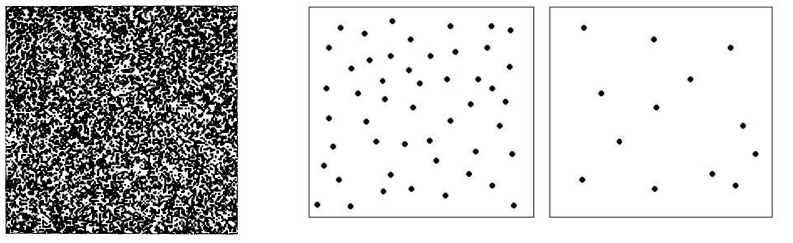
\includegraphics[width=0.6\textwidth]{helmholtz_principle}        
    \caption{Representation of the Helmholtz's principle: a) Uniform random imagen where no structure can be found. A group of five aligned dots exist in both images b) and c), but this structure can hardly be seen in the central image. Otherwise, in the right-most image the alignment stands out as an important deviation from randomness that cannot happen by chance and is therefore perceived.}\label{fig:helmholtz_principle}
\end{figure}


The Gestalt theory \citep{Wertheimer:Psycologische:1923} states that we can build a whole (gestalt) through the grouping of non-accidental detected primitives. That is, the human mind recognizes objects as a whole before examining their individual parts and the information that is not related in size, shape, orientation, etc., is perceived by the observer as chaotic and disorganized. The grouping of individual elements in a whole follows a set of laws defined by the Gestalt theory; some of them are (see Fig. \ref{fig:gestalt_laws}):

\begin{itemize}
	\item Similarity law
	\item Proximity law
	\item Continuity law
	\item Closure law
	\item Connectedness law
	\item Figure-ground law
	
\end{itemize}

\begin{figure}[!ht]
    \centering
    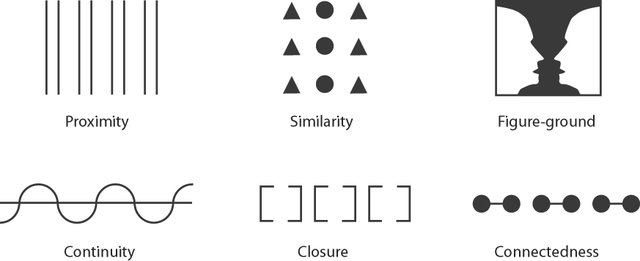
\includegraphics[width=0.6\textwidth]{gestalt_laws}        
    \caption{Representation of the Gestalt's law of grouping.}\label{fig:gestalt_laws}
\end{figure}

In this work, we explore the above ideas and propose a novel approach to detect a landing target in the same way as humans do, imitating the human perception process. To achieve this, we use the image contours retrieved at different scales. From this set of contours, we obtain the most perceptual contours, that is, those that were not generated by chance using an a contrario approach. After this, we take advantage of the predefined form of the targets to propose some measures that represent the laws of grouping of similarity and proximity of the Gestalt. Finally, we do the decoding and correction of target identification errors using Hamming's code. The diagram shown in the figure \ref{fig:target_detection_pipeline} groups the stages of our method for the perceptual detection of landing targets.

\begin{figure}[!ht]
    \centering
    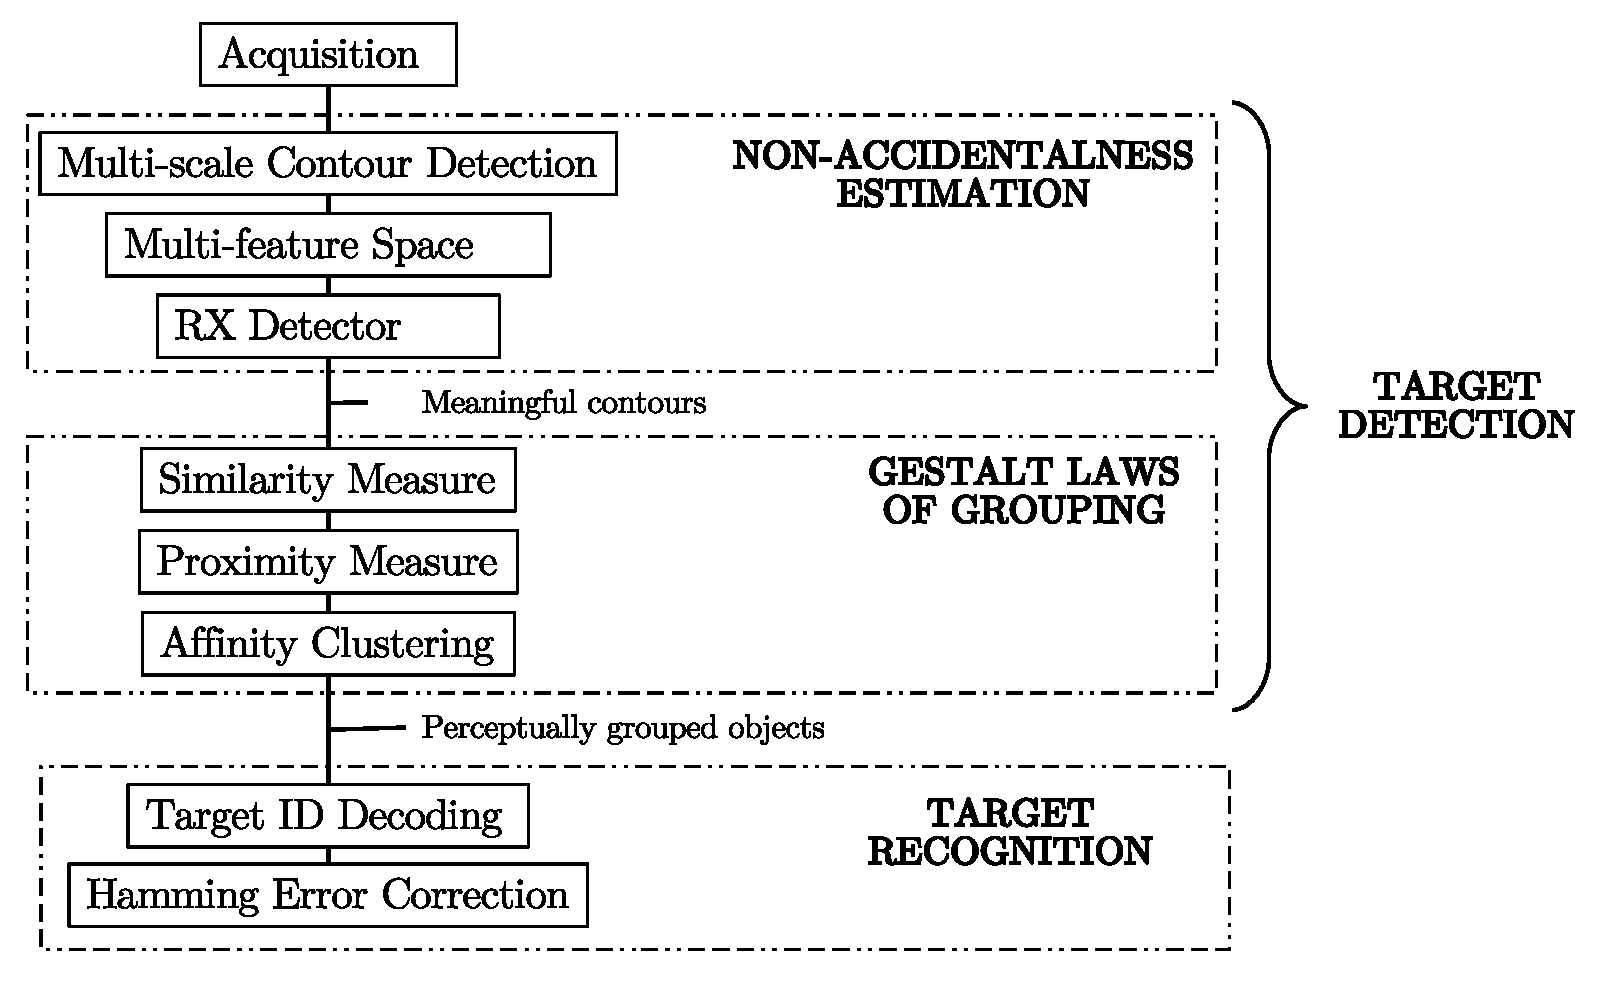
\includegraphics[width=\textwidth]{target_detection_pipeline}        
    \caption{Diagram of the phases for the landing target detection and recognition}\label{fig:target_detection_pipeline}
\end{figure}

The following sections are devoted to detailing the framework for the detection of landing targets. In section \ref{sec:hierarchical_target_detection} we evaluate different threshold-based methods for obtaining contours in an algorithm that uses the hierarchy of contours for the detection of landing targets. After that, we develop our perception model in section \ref{sec:unsupervised_perception_model}. Specifically, subsection \ref{subsec:Helmholtz} describes how to retrieve image contours as meaningful primitives and subsection \ref{subsec:Gestalt} describes how to group the contours to detect a landing target perceptually.  Later, in section \ref{sec:validation_and_test} we present the implementation of our methodology and some tests with both, synthetic and real-life images. We also present some conclusion and perspectives in section \ref{sec:conclusions_landing_target}. Finally, the appendix \ref{ch:target_description} contains the description of the landing target as well as the strategy used for its generation.


\section{Hierarchical Countours for Target Detection}\label{sec:hierarchical_target_detection}

Originally, the idea of landing targets detection is inspired by the needs of the Internest company \citep{InternestWeb}. The objective is to design a landing marker and an algorithm for its detection; all of this in the context of the UAV's autonomous precision landing task. 
A first approach, developed during during the traineeship period of a master student \citep{BaquedanoA.:ESIEE:2017}, seeks to solve the task straightforwardly using highly studied techniques. The algorithm is based on finding the contours of a binary image generated by the threshold method proposed by Otsu \citep{Otsu:SMC:1979}. Since the landing target they propose is composed of nested concentric circles, they heuristically use the hierarchy of the found contours to detect a landing target. Their methodology consists in discriminating the contours that are not nested through conditional evaluations at each hierarchy level. The conditions are hierarchically dependent which means that the landing target detection is frustrated if the conditions are not strictly enforced.

This idea was tested, however, similarly to some other works mentioned in section \ref{sec:introduction_ch1}, the algorithm works well only under certain circumstances. The tests show that the algorithm fails mainly because it is not able to find all the target contours. This generally occurs when the landing target is exposed to conditions that degrade the quality of the image. Given the nature of the aerial object detection task, factors such as the change in height and orientation of the UAV, modify the perception of an object introducing disturbances such as noise, changes in lighting and contrast, deformation of objects, etc., that complicate the operation of threshold-based and consequently the contour detection. We classify the disturbances suffered by landing targets into four types: 

\begin{enumerate}
	\item Change in size w.r.t. the scene.
	\item Presence of noise.
	\item Presence of shadows.
	\item Deformation due to perspective.
\end{enumerate}

Figure \ref{fig:tar_degradations} shows a the landing target affected by the aforementioned disturbances.
  
\begin{figure}[!ht]
    \centering
    \begin{subfigure}[b]{0.3\textwidth}
        \frame{
\includegraphics[width=\textwidth]{tar_noise}}
        \caption{}
        \label{fig:deg_noise}
    \end{subfigure}
        ~ %add desired spacing between images, e. g. ~, \quad, \qquad, \hfill etc. 
      %(or a blank line to force the subfigure onto a new line)
    \begin{subfigure}[b]{0.3\textwidth}
        \frame{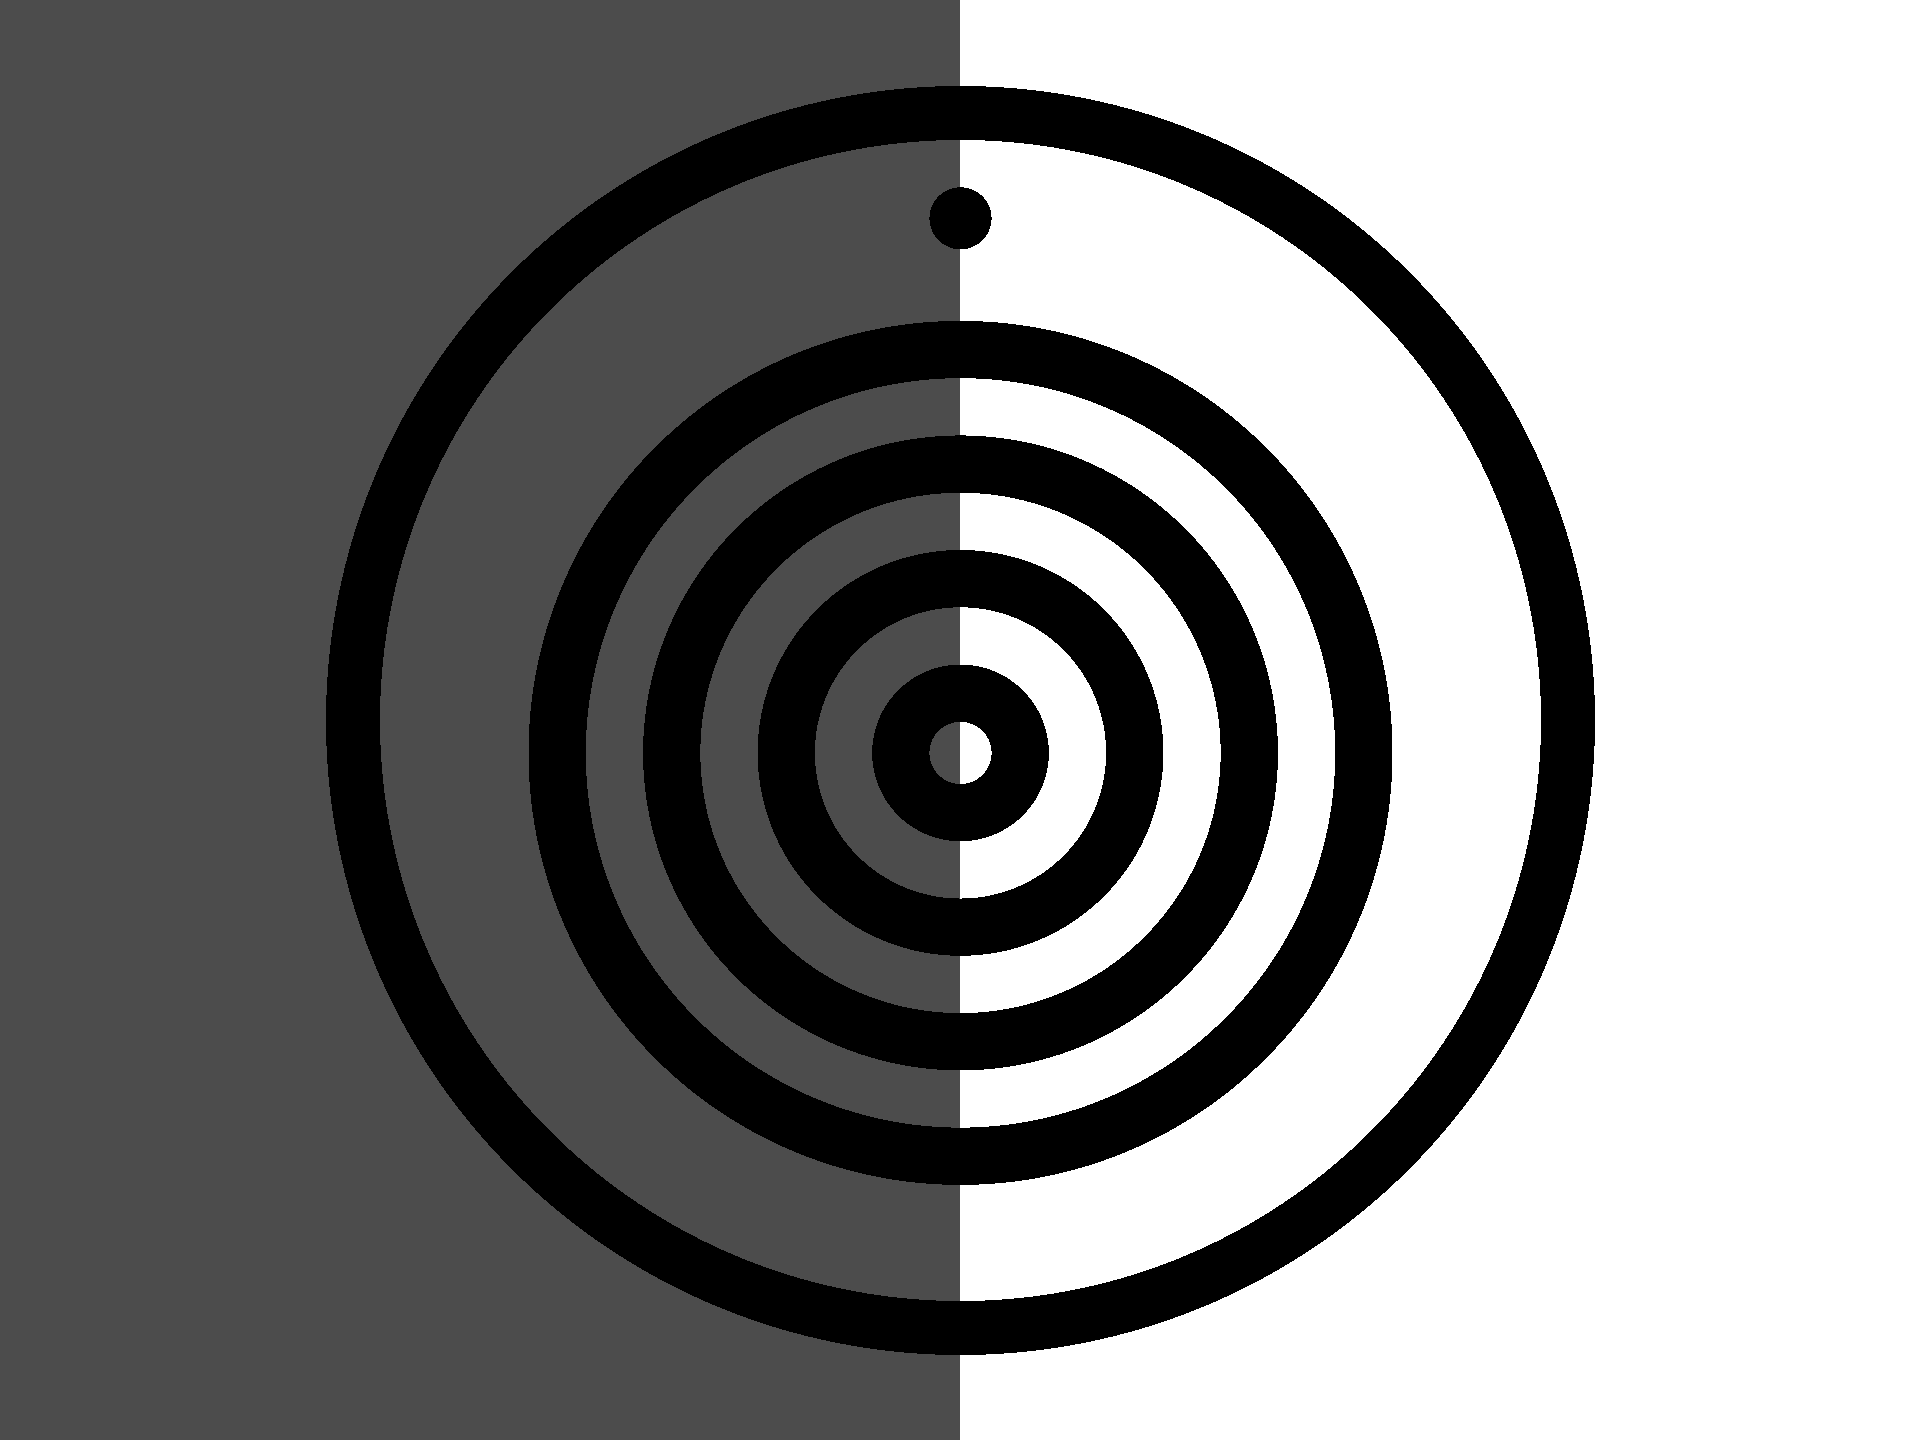
\includegraphics[width=\textwidth]{tar_shadow}}
        \caption{}
        \label{fig:deg_shadow}
    \end{subfigure}\\
        ~ %add desired spacing between images, e. g. ~, \quad, \qquad, \hfill etc. 
      %(or a blank line to force the subfigure onto a new line)
    \begin{subfigure}[b]{0.3\textwidth}
        \frame{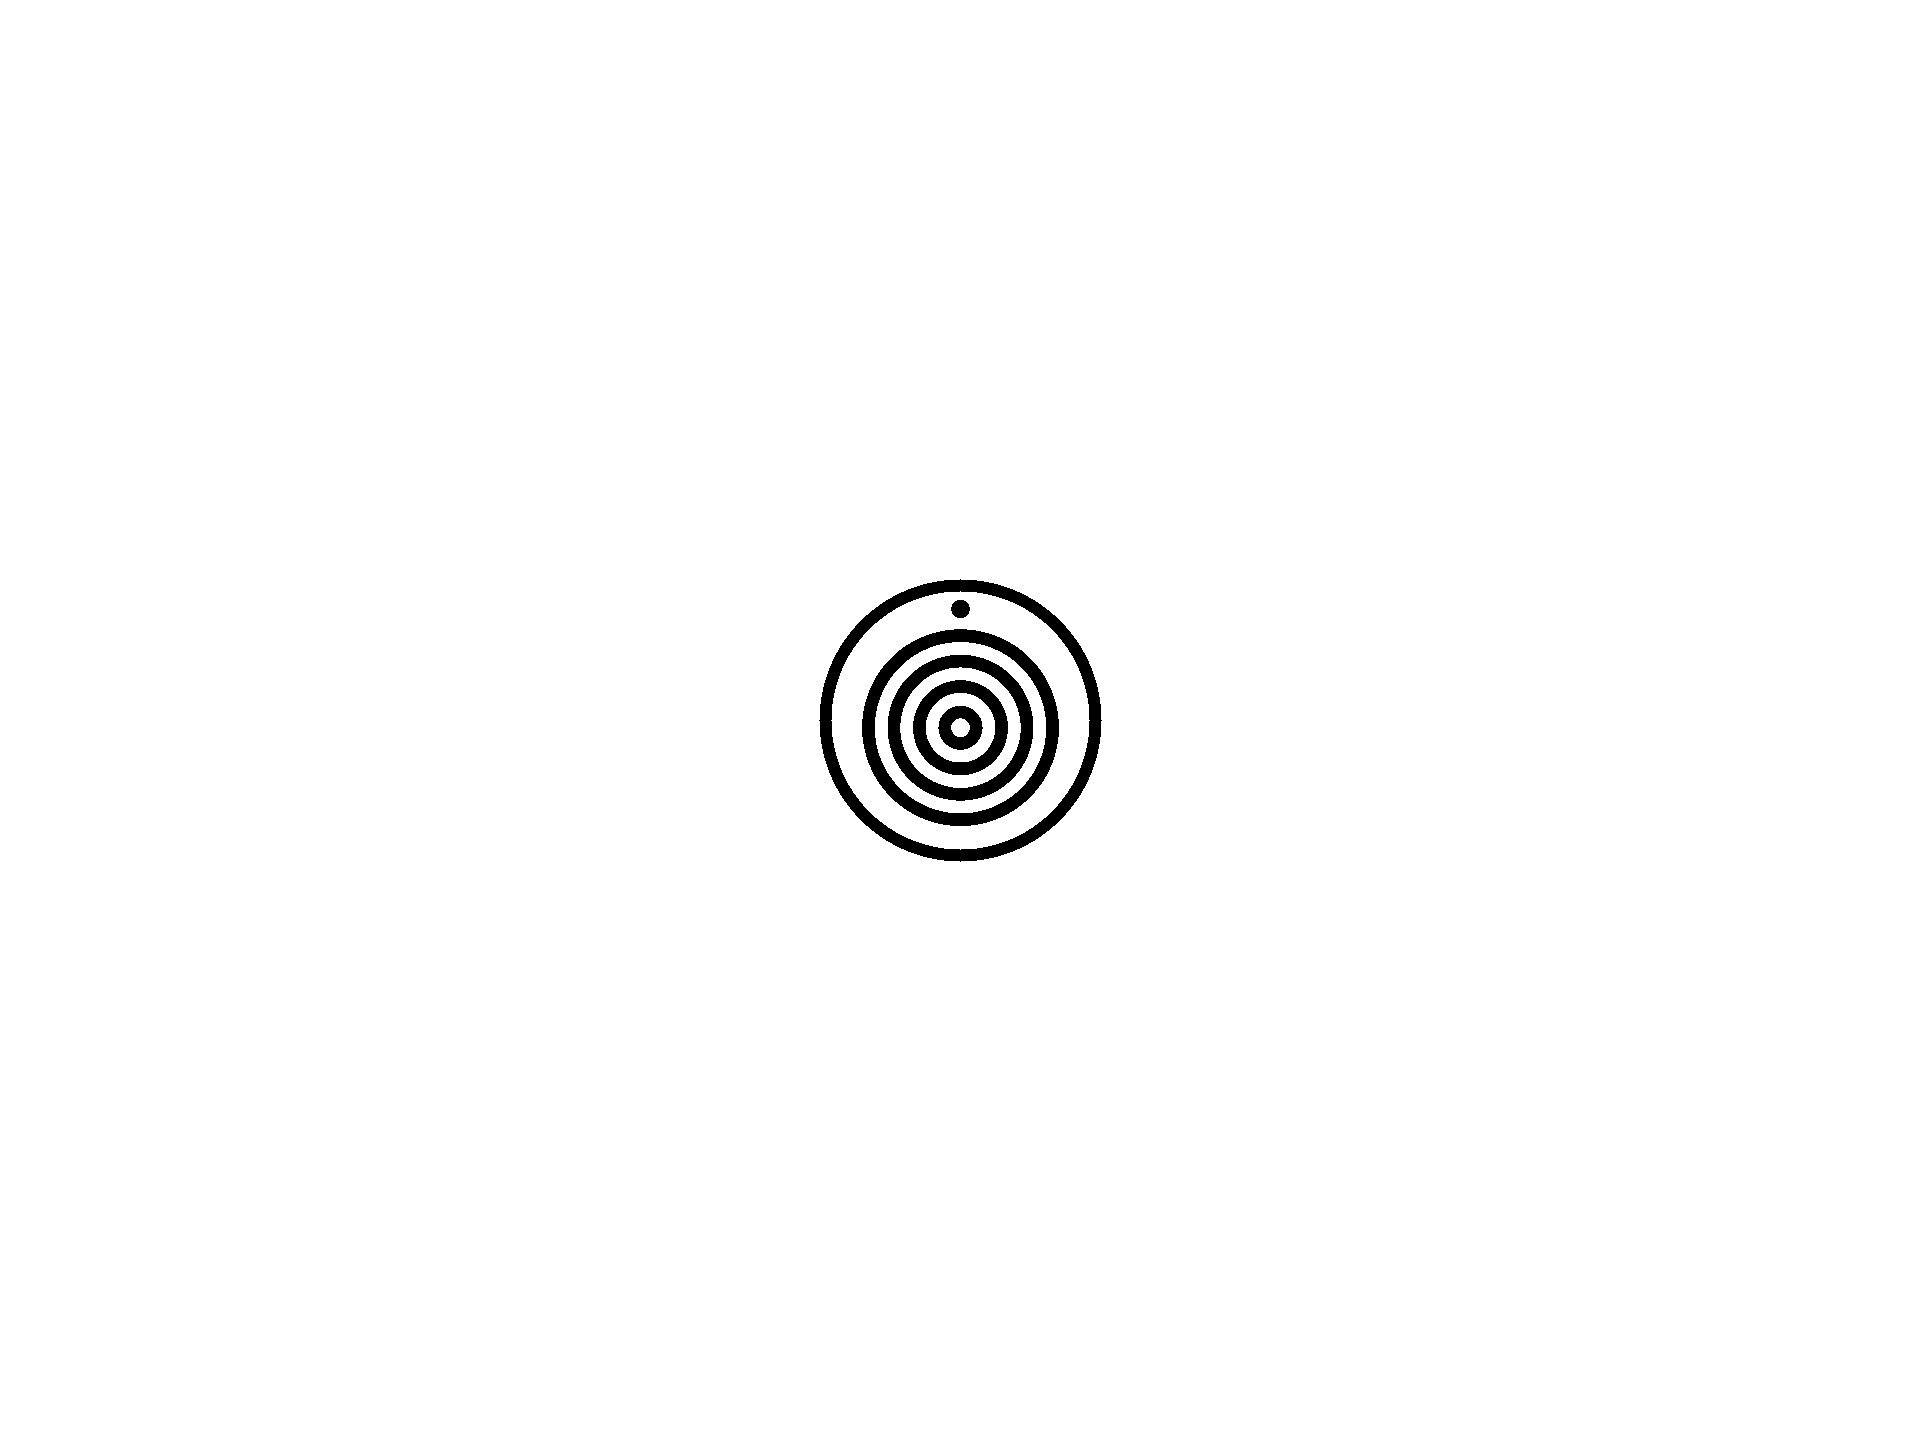
\includegraphics[width=\textwidth]{tar_resolution}}
        \caption{}
        \label{fig:deg_resolution}
    \end{subfigure}
        ~ %add desired spacing between images, e. g. ~, \quad, \qquad, \hfill etc. 
      %(or a blank line to force the subfigure onto a new line)
    \begin{subfigure}[b]{0.3\textwidth}
        \frame{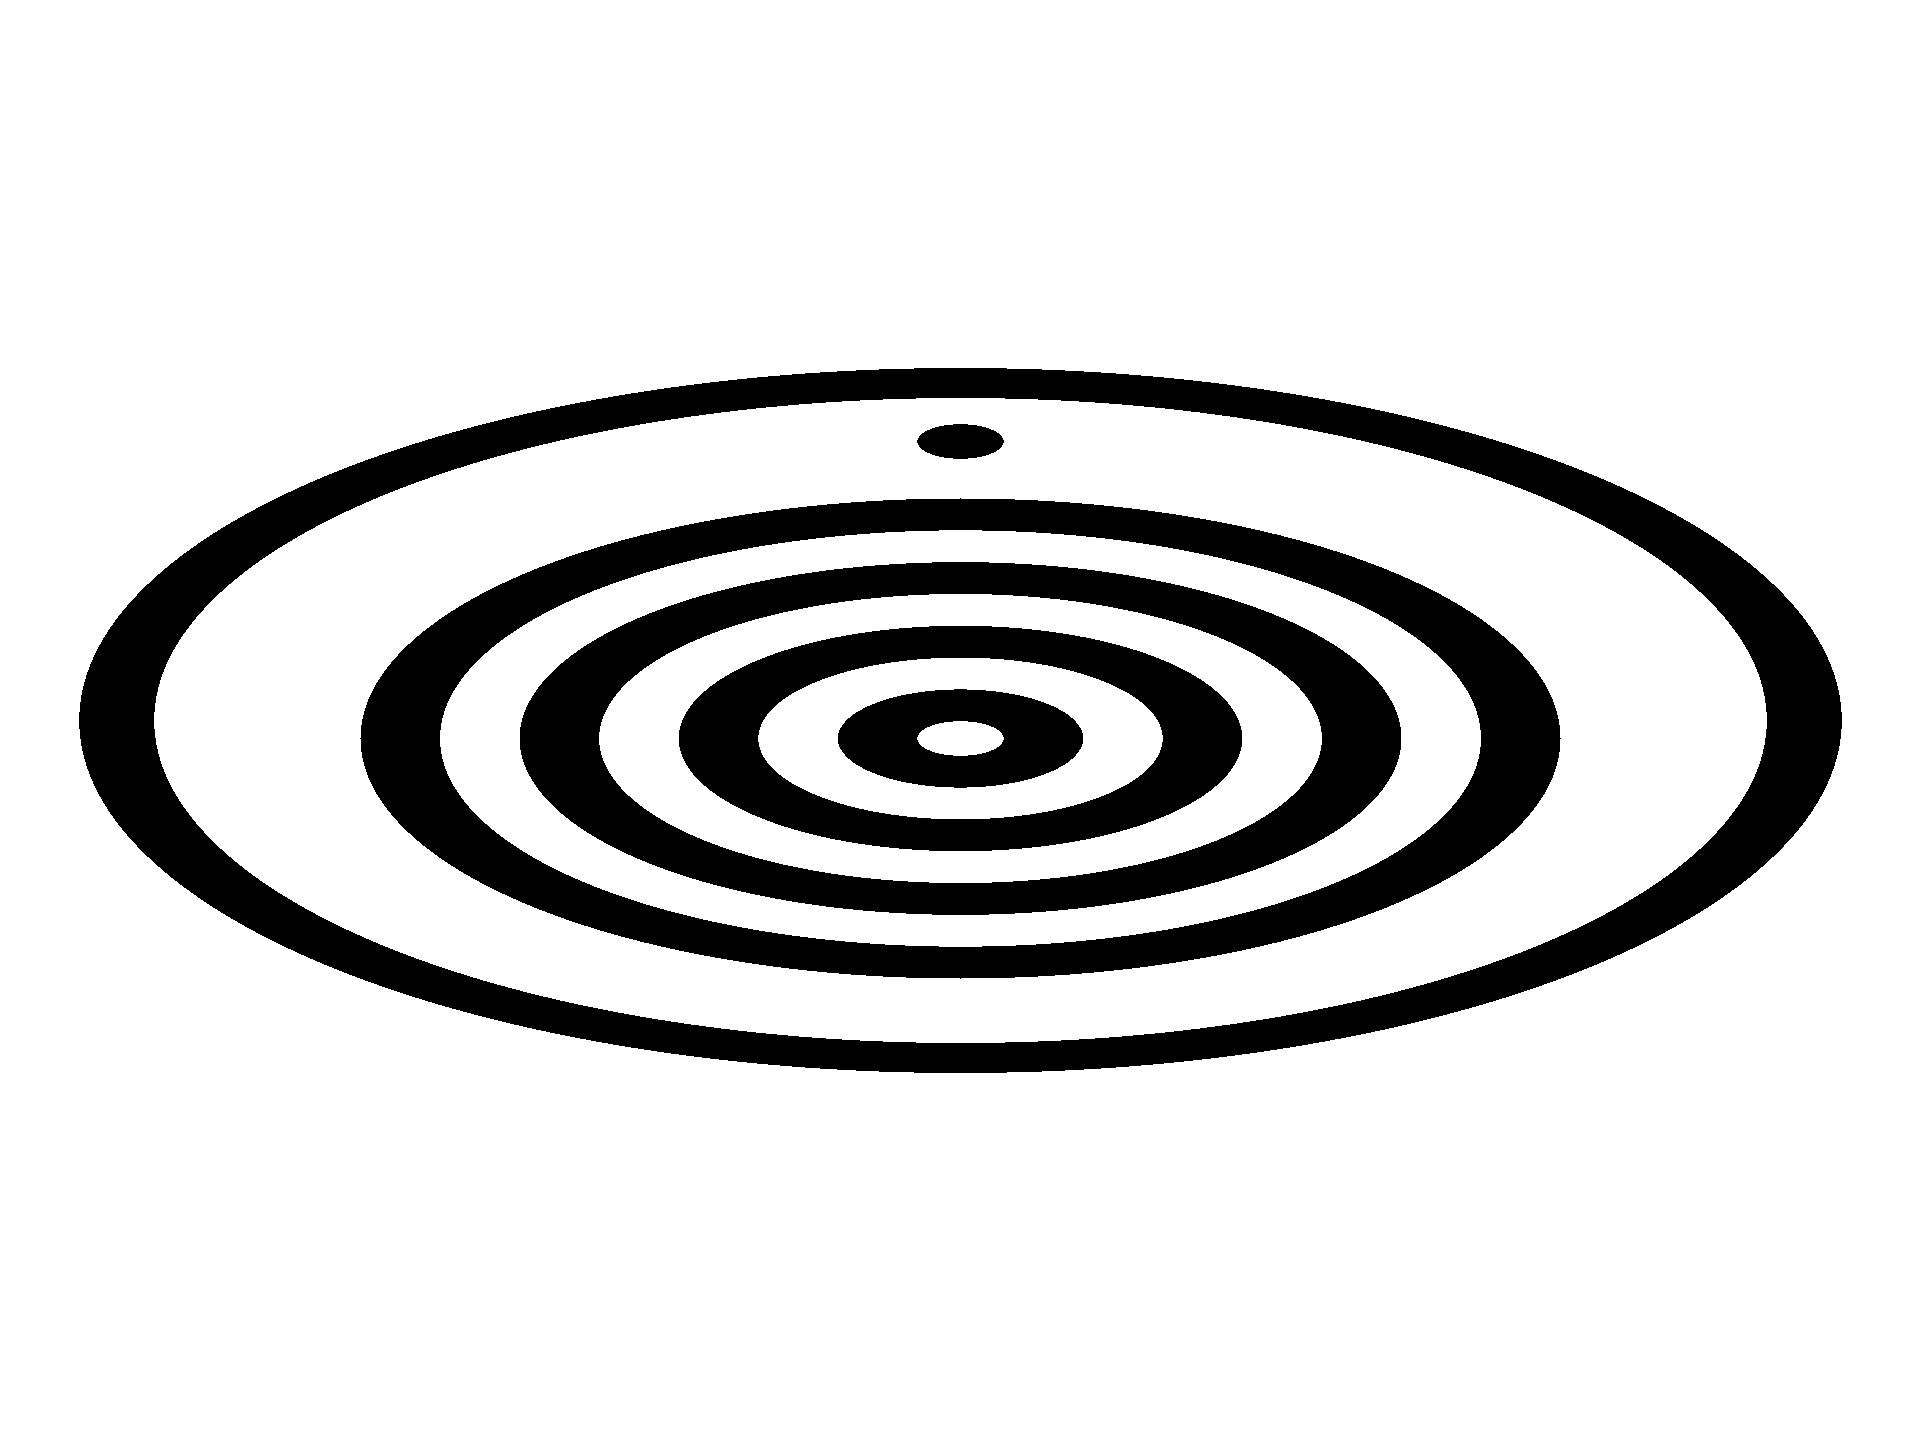
\includegraphics[width=\textwidth]{tar_deformation}}
        \caption{}
        \label{fig:deg_deformation}
    \end{subfigure}
    \caption{ Landing target degradations: \textbf{(a)} Noise, \textbf{(b)} Shadow, \textbf{(c)} Change of size and \textbf{(d)} Perspectice deformation}\label{fig:tar_degradations}
\end{figure}

One of the main disadvantages of the hierarchy method for the detection of landing targets is that its effectiveness lies with the Otsu contour detector, which does not work well in images with high contrast or severe changes in lighting. However, there are other threshold-based methods for contour detection that could better face the image degradations showed in figure \ref{fig:tar_degradations}. Following the taxonomy for threshold-based methods proposed in \citep{Sezgin.Sankur:EI:2010}, there are clustering-based methods such as Otsu \citep{Otsu:SMC:1979} and the Riddler \citep{Ridler.Calvard:TSMC:1978}; the entropy-based such as Yen\citep{Yen.Chang.ea:TIP:1995} and Li\citep{Li.Lee:ICPR:1993}; local methods such as Niblack \citep{Niblack:ImageProcc:1986} and Sauvla \citep{Sauvola.Pietikainen:ICPR:2000}; the adaptive method proposed by Bradley \citep{Bradley.Roth:ACM:2007} and finally, the mean and Gaussian pixel distribution as spacial methods. 
We use these nine representative threshold-based methods to obtain a binary image, localize the image contours and evaluate which is the best facing image degradations showed in figure \ref{fig:tar_degradations}.


\begin{figure}[htbp]
\centering
\begin{subfigure}[t]{\dimexpr0.15\textwidth+20pt\relax}
    \makebox[20pt]{\raisebox{30pt}{\rotatebox[origin=c]{90}{Input}}}%Input (zoom)
    \frame{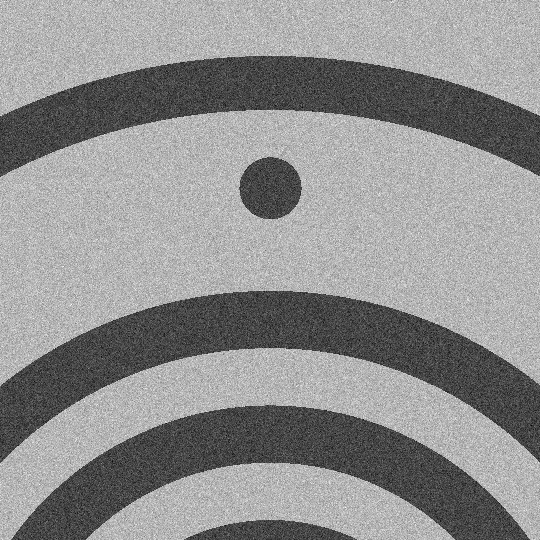
\includegraphics[width=\dimexpr\linewidth-20pt\relax]
    {tar_zoom_noise}}
    \makebox[20pt]{\raisebox{30pt}{\rotatebox[origin=c]{90}{Otsu}}}%
    \frame{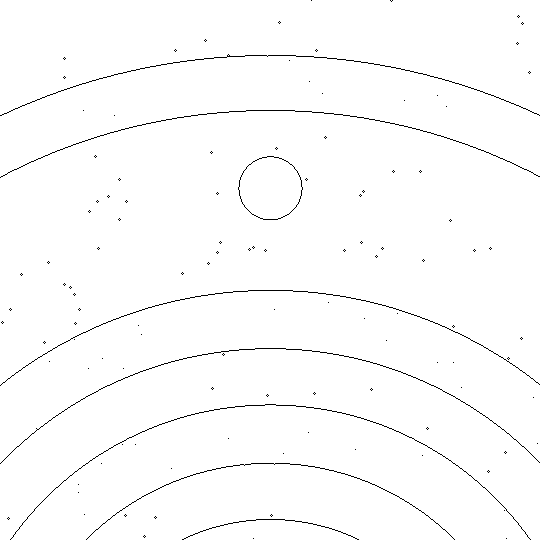
\includegraphics[width=\dimexpr\linewidth-20pt\relax]
    {Otsu_cont_noise}}
    \makebox[20pt]{\raisebox{30pt}{\rotatebox[origin=c]{90}{Riddler}}}%
    \frame{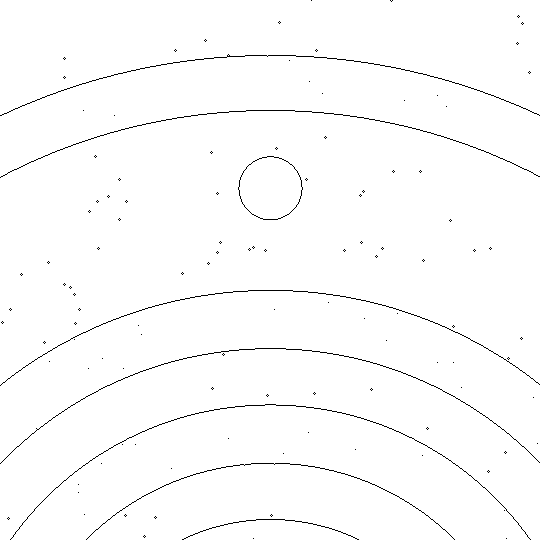
\includegraphics[width=\dimexpr\linewidth-20pt\relax]
    {Riddler_cont_noise}}
    \makebox[20pt]{\raisebox{30pt}{\rotatebox[origin=c]{90}{Yen}}}%
    \frame{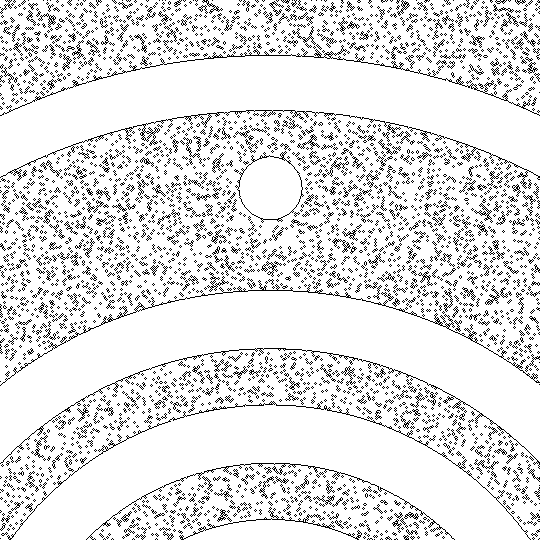
\includegraphics[width=\dimexpr\linewidth-20pt\relax]
    {Yen_cont_noise}}
    \makebox[20pt]{\raisebox{30pt}{\rotatebox[origin=c]{90}{Li}}}%
    \frame{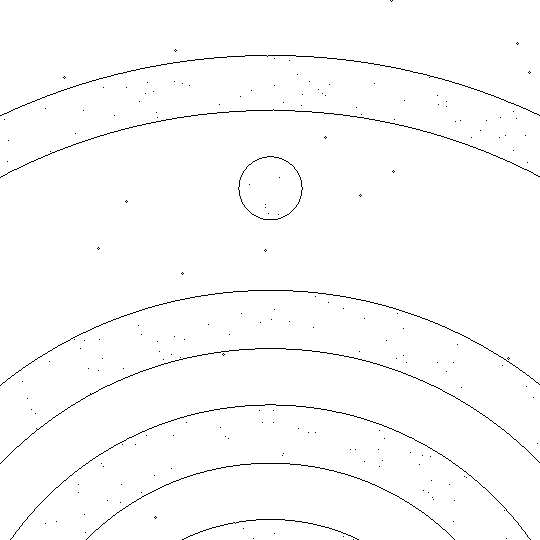
\includegraphics[width=\dimexpr\linewidth-20pt\relax]
    {Li_cont_noise}}
    \makebox[20pt]{\raisebox{30pt}{\rotatebox[origin=c]{90}{Niblack}}}%
    \frame{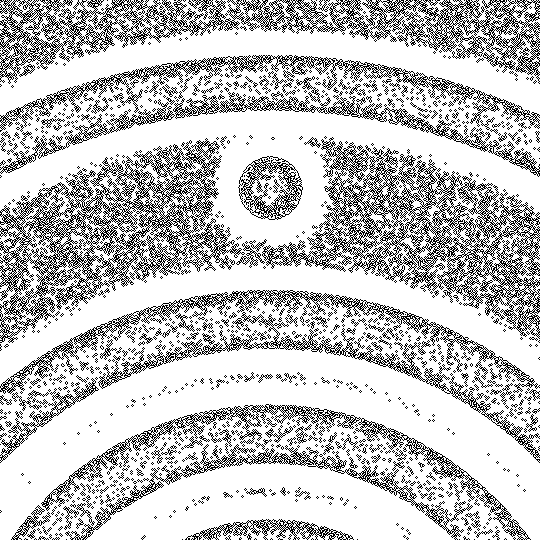
\includegraphics[width=\dimexpr\linewidth-20pt\relax]
    {Niblack_cont_noise}}
    \makebox[20pt]{\raisebox{30pt}{\rotatebox[origin=c]{90}{Sauvola}}}%
    \frame{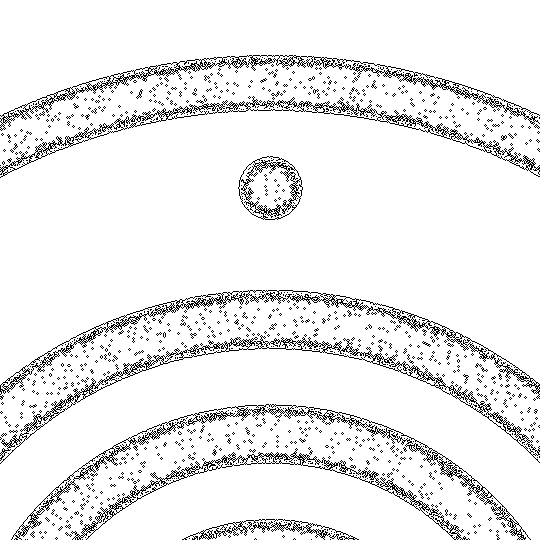
\includegraphics[width=\dimexpr\linewidth-20pt\relax]
    {Sauvola_cont_noise}}
    \makebox[20pt]{\raisebox{30pt}{\rotatebox[origin=c]{90}{Bradley}}}%
    \frame{
\includegraphics[width=\dimexpr\linewidth-20pt\relax]
    {Bradley_cont_noise}}
    \makebox[20pt]{\raisebox{30pt}{\rotatebox[origin=c]{90}{Gauss}}}%
    \frame{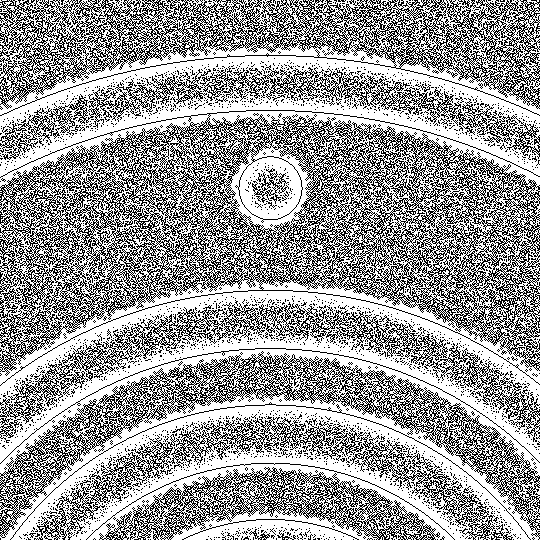
\includegraphics[width=\dimexpr\linewidth-20pt\relax]
    {Gauss_cont_noise}}
    \makebox[20pt]{\raisebox{30pt}{\rotatebox[origin=c]{90}{Mean}}}%
    \frame{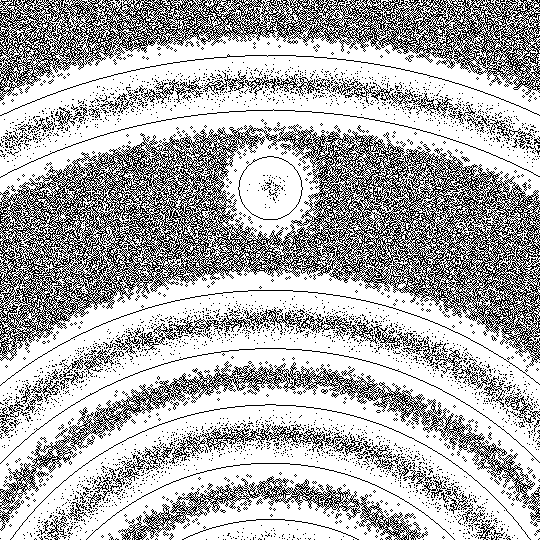
\includegraphics[width=\dimexpr\linewidth-20pt\relax]
    {Mean_cont_noise}}
    \caption{} 
\end{subfigure}\qquad
\begin{subfigure}[t]{0.15\textwidth}
    \frame{
\includegraphics[width=\textwidth]
    {tar_zoom_shadow}}
    \frame{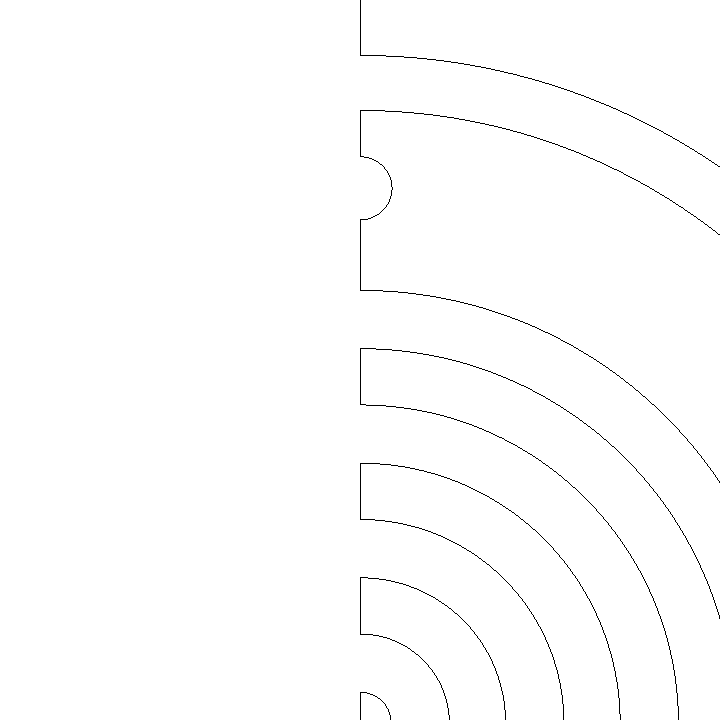
\includegraphics[width=\textwidth]
    {Otsu_cont_shadow}}
    \frame{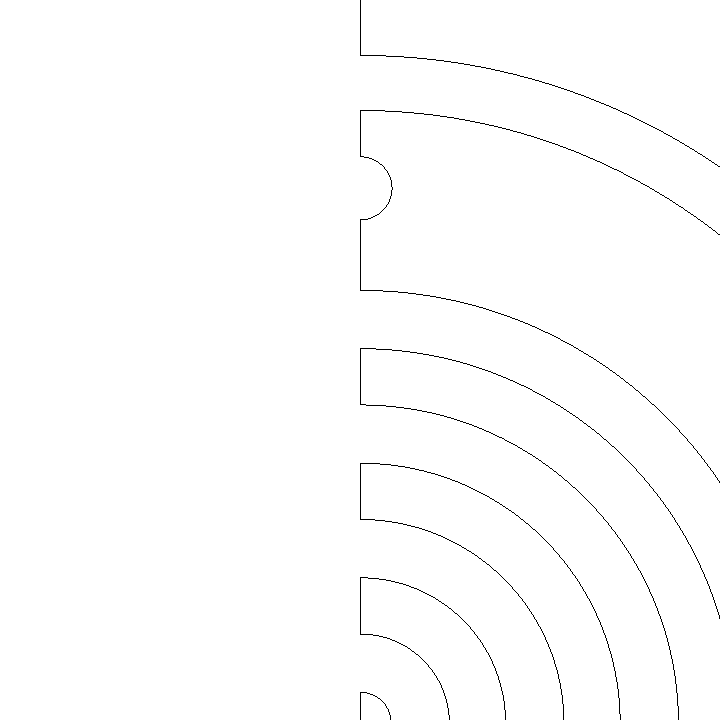
\includegraphics[width=\textwidth]
    {Riddler_cont_shadow}}
    \frame{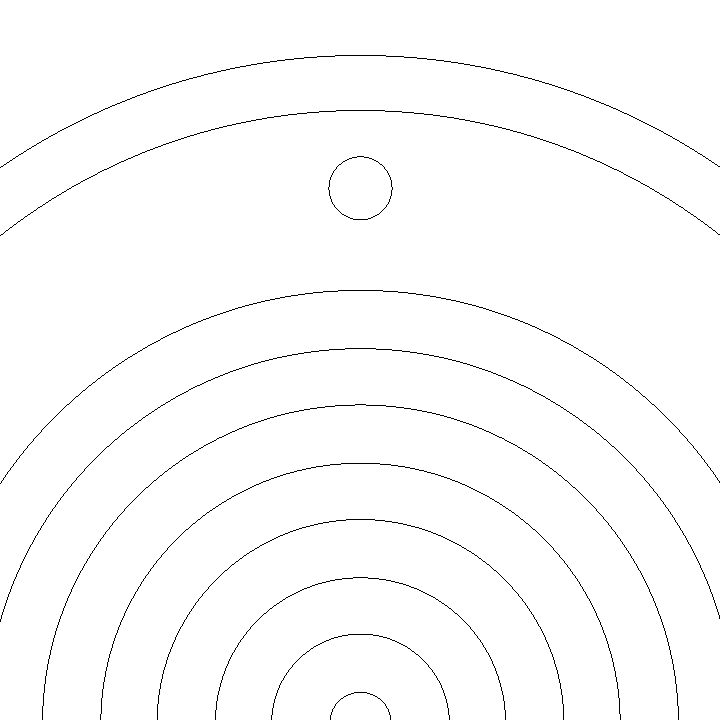
\includegraphics[width=\textwidth]
    {Yen_cont_shadow}}
    \frame{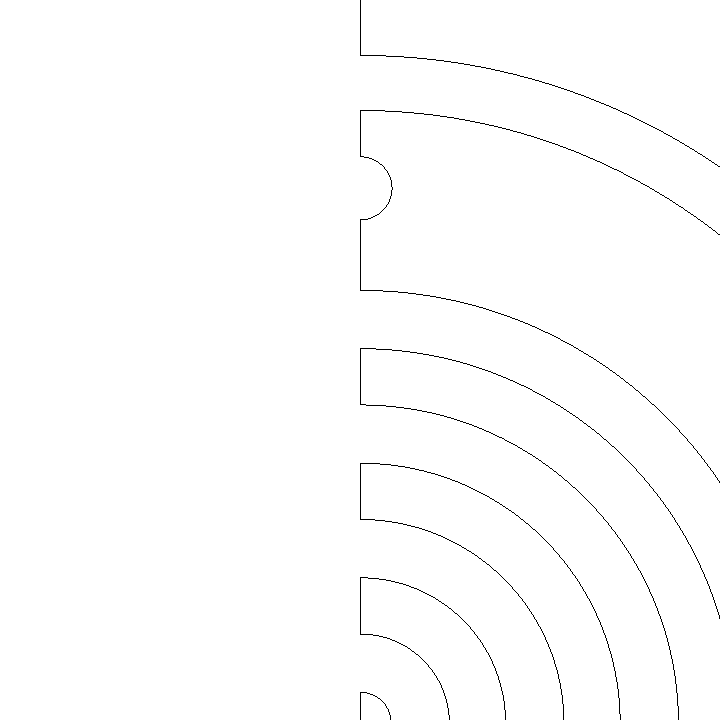
\includegraphics[width=\textwidth]
    {Li_cont_shadow}}
    \frame{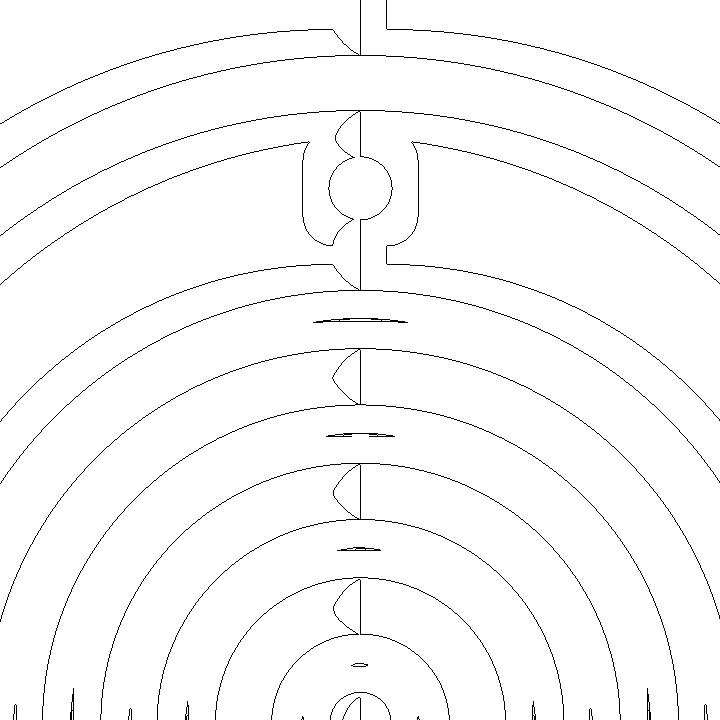
\includegraphics[width=\textwidth]
    {Niblack_cont_shadow}}
    \frame{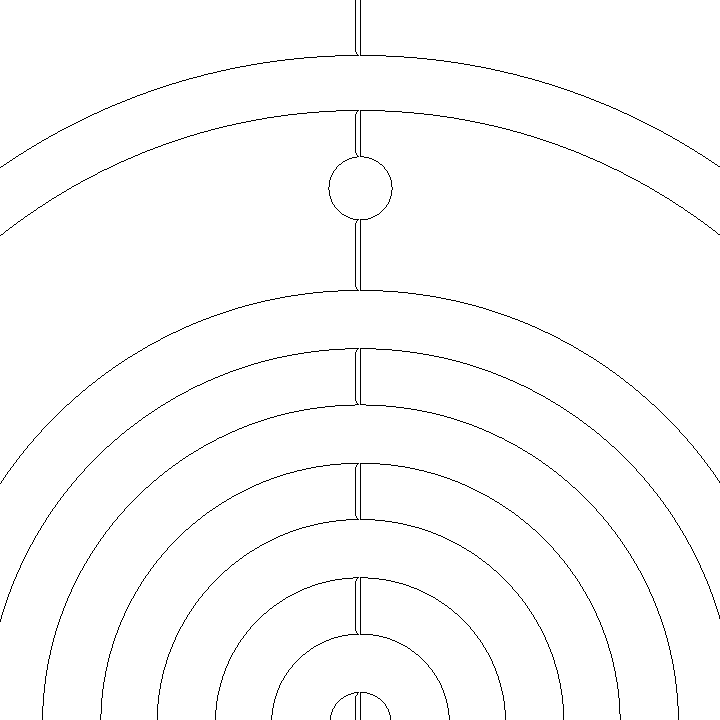
\includegraphics[width=\textwidth]
    {Sauvola_cont_shadow}}
    \frame{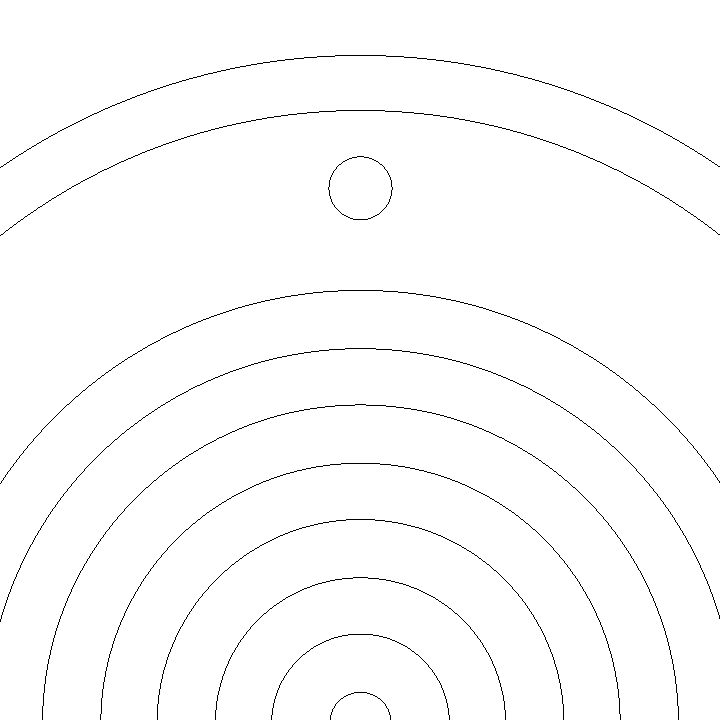
\includegraphics[width=\textwidth]
    {Bradley_cont_shadow}}
    \frame{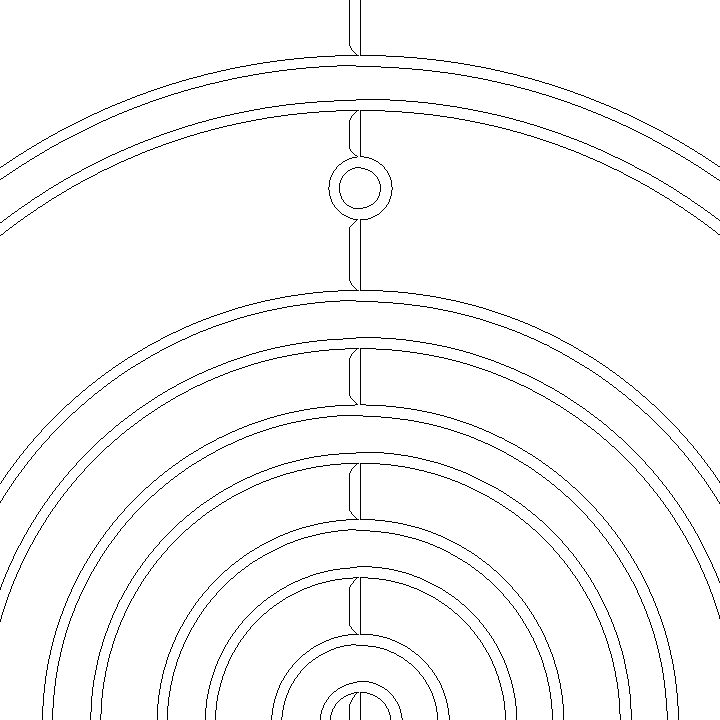
\includegraphics[width=\textwidth]
    {Gauss_cont_shadow}}
    \frame{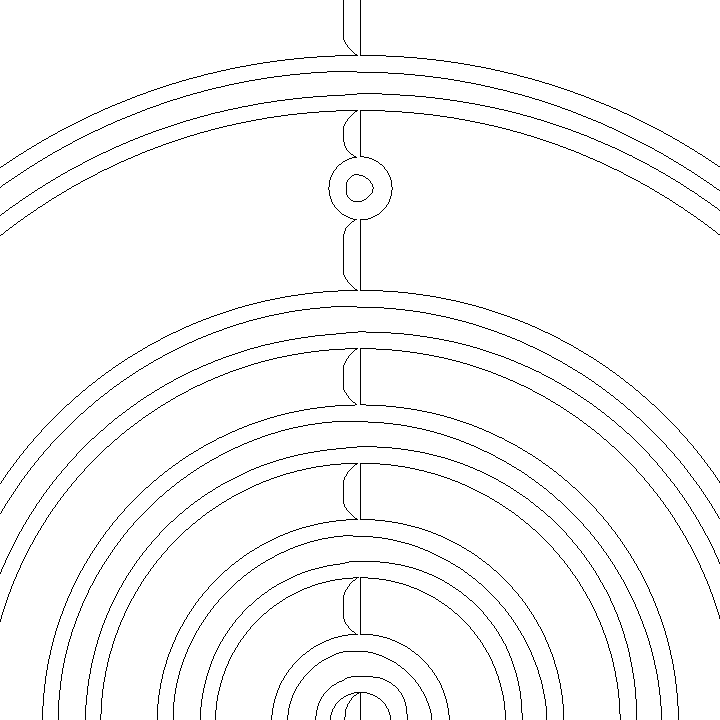
\includegraphics[width=\textwidth]
    {Mean_cont_shadow}}
    \caption{} 
\end{subfigure}\qquad
\begin{subfigure}[t]{0.15\textwidth}
    \frame{
\includegraphics[width=\textwidth]
    {tar_zoom_resolution}}
    \frame{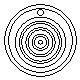
\includegraphics[width=\textwidth]
    {Otsu_cont_resolution}}
    \frame{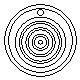
\includegraphics[width=\textwidth]
    {Riddler_cont_resolution}}
    \frame{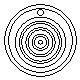
\includegraphics[width=\textwidth]
    {Yen_cont_resolution}}
    \frame{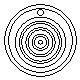
\includegraphics[width=\textwidth]
    {Li_cont_resolution}}
    \frame{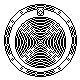
\includegraphics[width=\textwidth]
    {Niblack_cont_resolution}}
    \frame{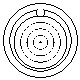
\includegraphics[width=\textwidth]
    {Sauvola_cont_resolution}}
    \frame{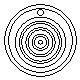
\includegraphics[width=\textwidth]
    {Bradley_cont_resolution}}
    \frame{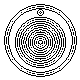
\includegraphics[width=\textwidth]
    {Gauss_cont_resolution}}
    \frame{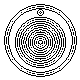
\includegraphics[width=\textwidth]
    {Mean_cont_resolution}}
    \caption{} 
\end{subfigure}\qquad
\begin{subfigure}[t]{0.15\textwidth}
    \frame{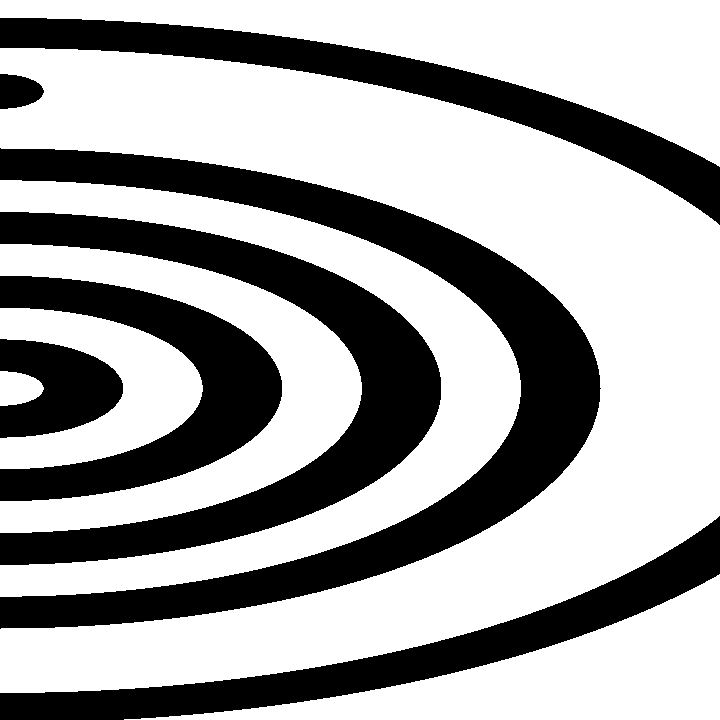
\includegraphics[width=\textwidth]
    {tar_zoom_deformation}}
    \frame{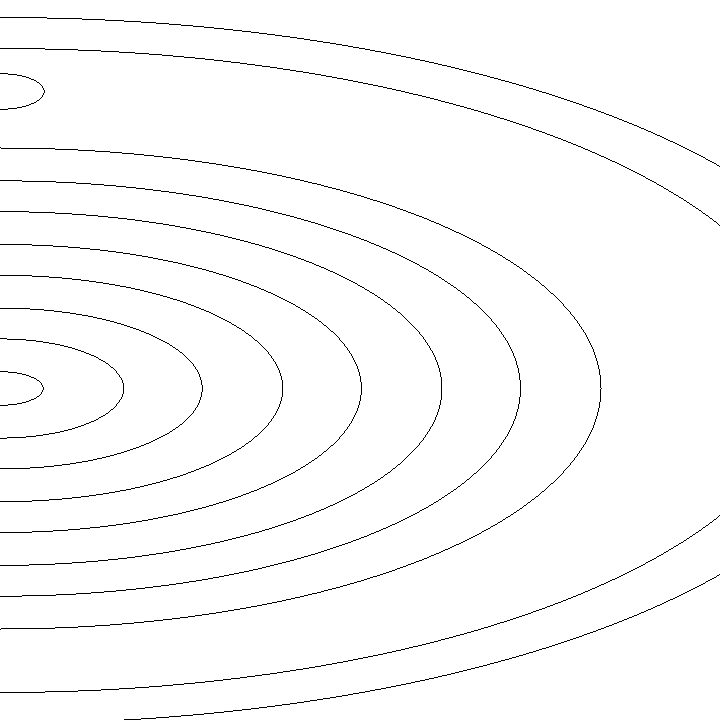
\includegraphics[width=\textwidth]
    {Otsu_cont_deformation}}
    \frame{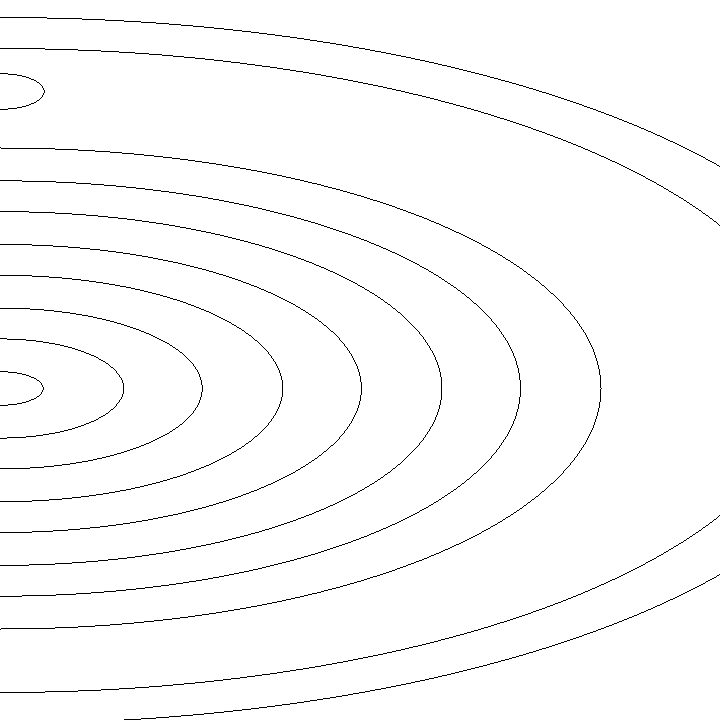
\includegraphics[width=\textwidth]
    {Riddler_cont_deformation}}
    \frame{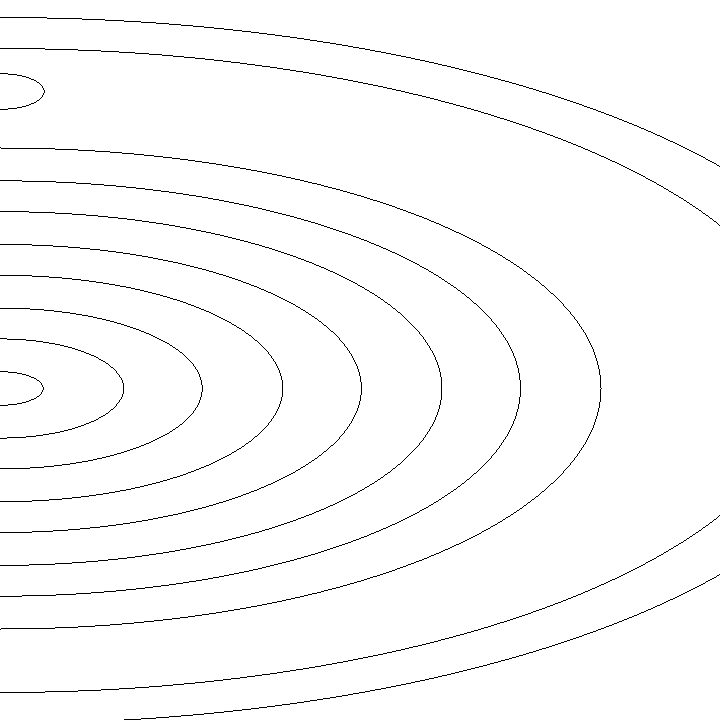
\includegraphics[width=\textwidth]
    {Yen_cont_deformation}}
    \frame{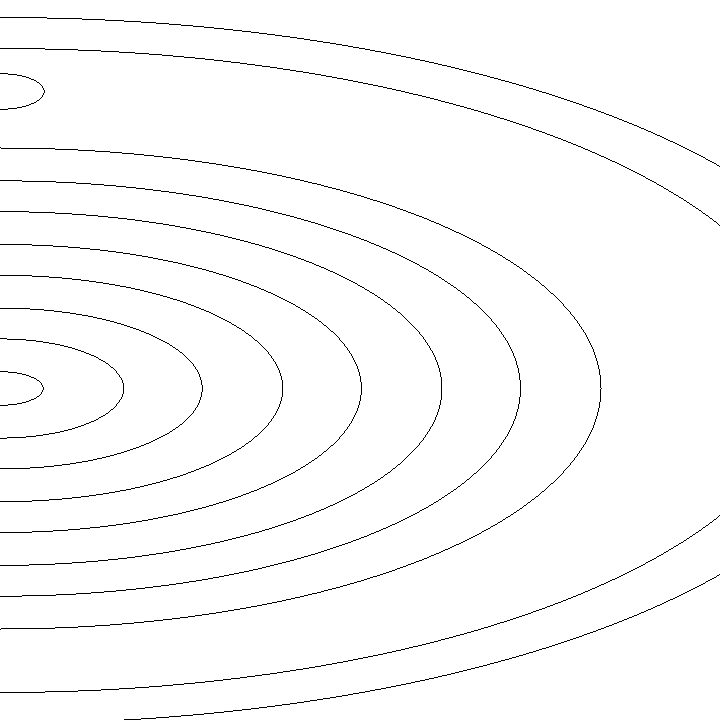
\includegraphics[width=\textwidth]
    {Li_cont_deformation}}
    \frame{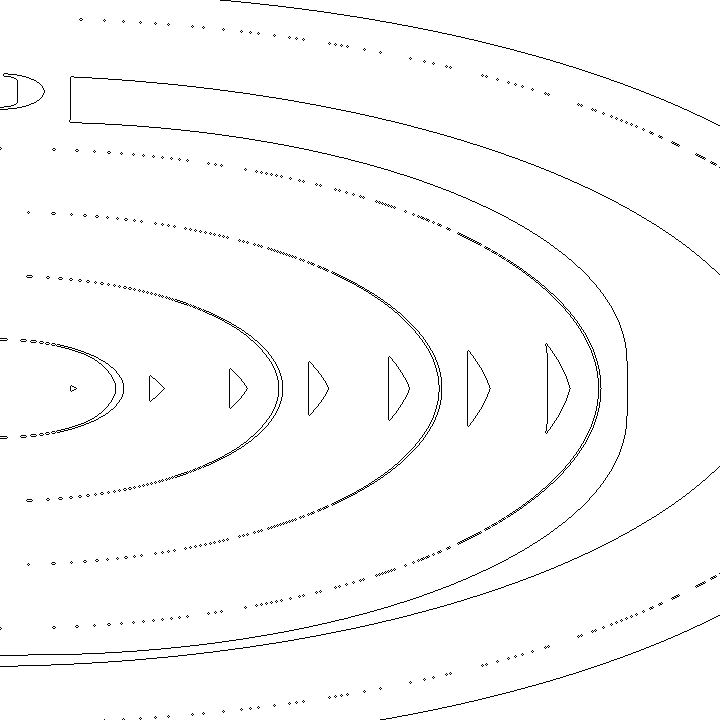
\includegraphics[width=\textwidth]
    {Niblack_cont_deformation}}
    \frame{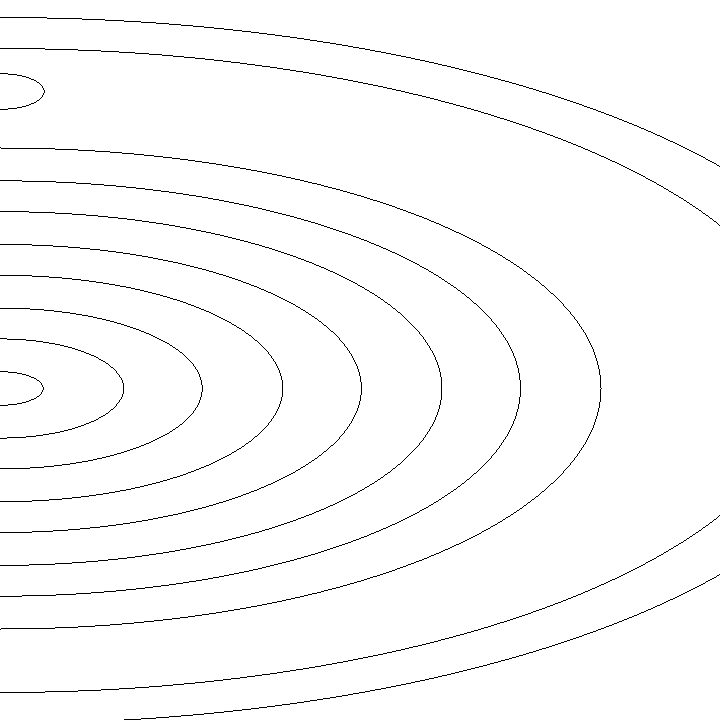
\includegraphics[width=\textwidth]
    {Sauvola_cont_deformation}}
    \frame{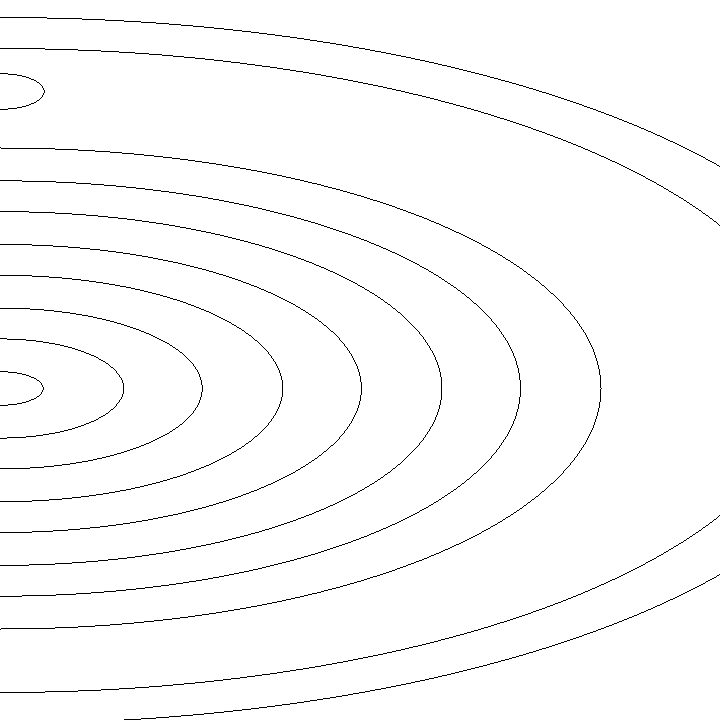
\includegraphics[width=\textwidth]
    {Bradley_cont_deformation}}
    \frame{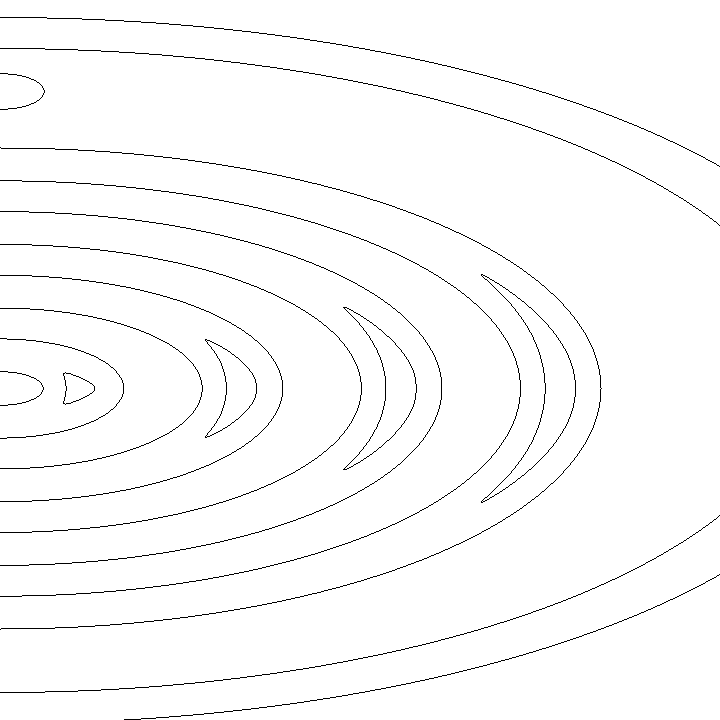
\includegraphics[width=\textwidth]
    {Gauss_cont_deformation}}
    \frame{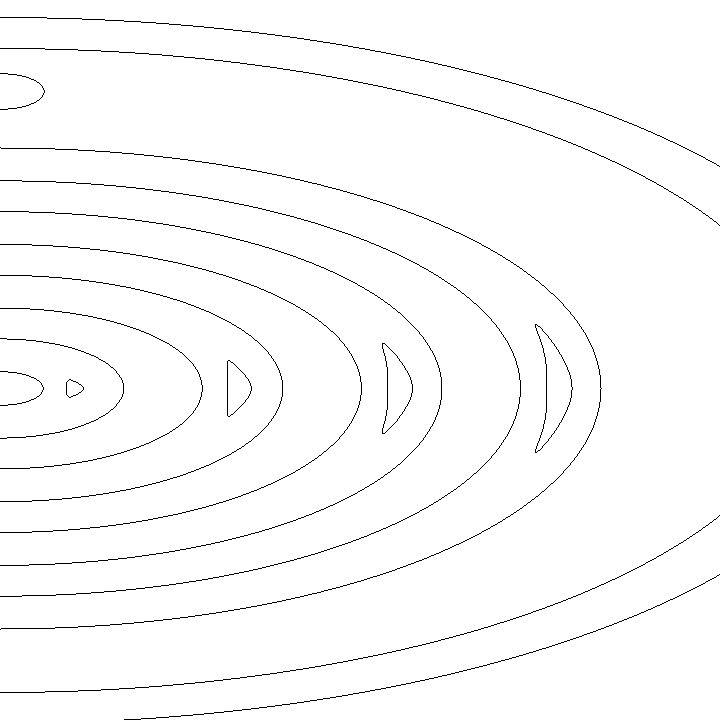
\includegraphics[width=\textwidth]
    {Mean_cont_deformation}}
    \caption{}  
\end{subfigure}
\caption{threshold-based methods result illustrations on synthetic images: \textbf{(a)} Noise, \textbf{(b)} Shadow, \textbf{(c)} Size and \textbf{(d)} Deformation degradations}\label{fig:thr_synth_comparison}
\end{figure}

The contours obtained applying each threshold-based method are depicted in figure \ref{fig:thr_synth_comparison}. In this figure is appreciable that, depending on the situation the result is better or worse. However, at first glance, there is not one that works correctly in a general way.

\subsection{Thershold-based Method's Evaluation}


We run the hierarchical algorithm proposed in \citep{BaquedanoA.:ESIEE:2017} on a database of synthetic images. The database contains the sixteen different landing targets perturbed by the image degradations of figure \ref{fig:tar_degradations}. 
The noise degradation is simulated by adding Gaussian noise with a mean of zero and a variable standard deviation from 0.02 to 0.2 where 0.02 is the minimum noise addition. The shadow perturbation is simulated shading the left-half of the image; the variation of the shadow is done between 0 and 1 where 0 indicates a darker left-half image. The last two degradations are related with the perspective and distance of the viewer (the camera). First, the change of scale is done scaling the landing target circles on a $640\times480$p image in an interval from 0 to 1, where 1 indicates real scale. Lastly, the perspective degradation is achieved by augmenting the proportion of one axis in an interval between 1 and 2, where to indicates the maximum deformation. We apply the maximum value degradation for the test.
 
We use the F1-score as metric to evaluate the accuracy of each threshold-based method under different degradations. This metric has values between 0 and 1, where 1 is the best score and 0 the worst. Figure \ref{fig:degradations_graphs} shows the F1-score of the threshold-based methods under the image degradations. The graphs show the behavior of the algorithm without an error-correction (gray bars) and with the use of the error-correction (black bars) described in appendix \ref{ch:target_description}.
\begin{figure}[h!]
    \centering
    \begin{subfigure}[b]{0.4\textwidth}
        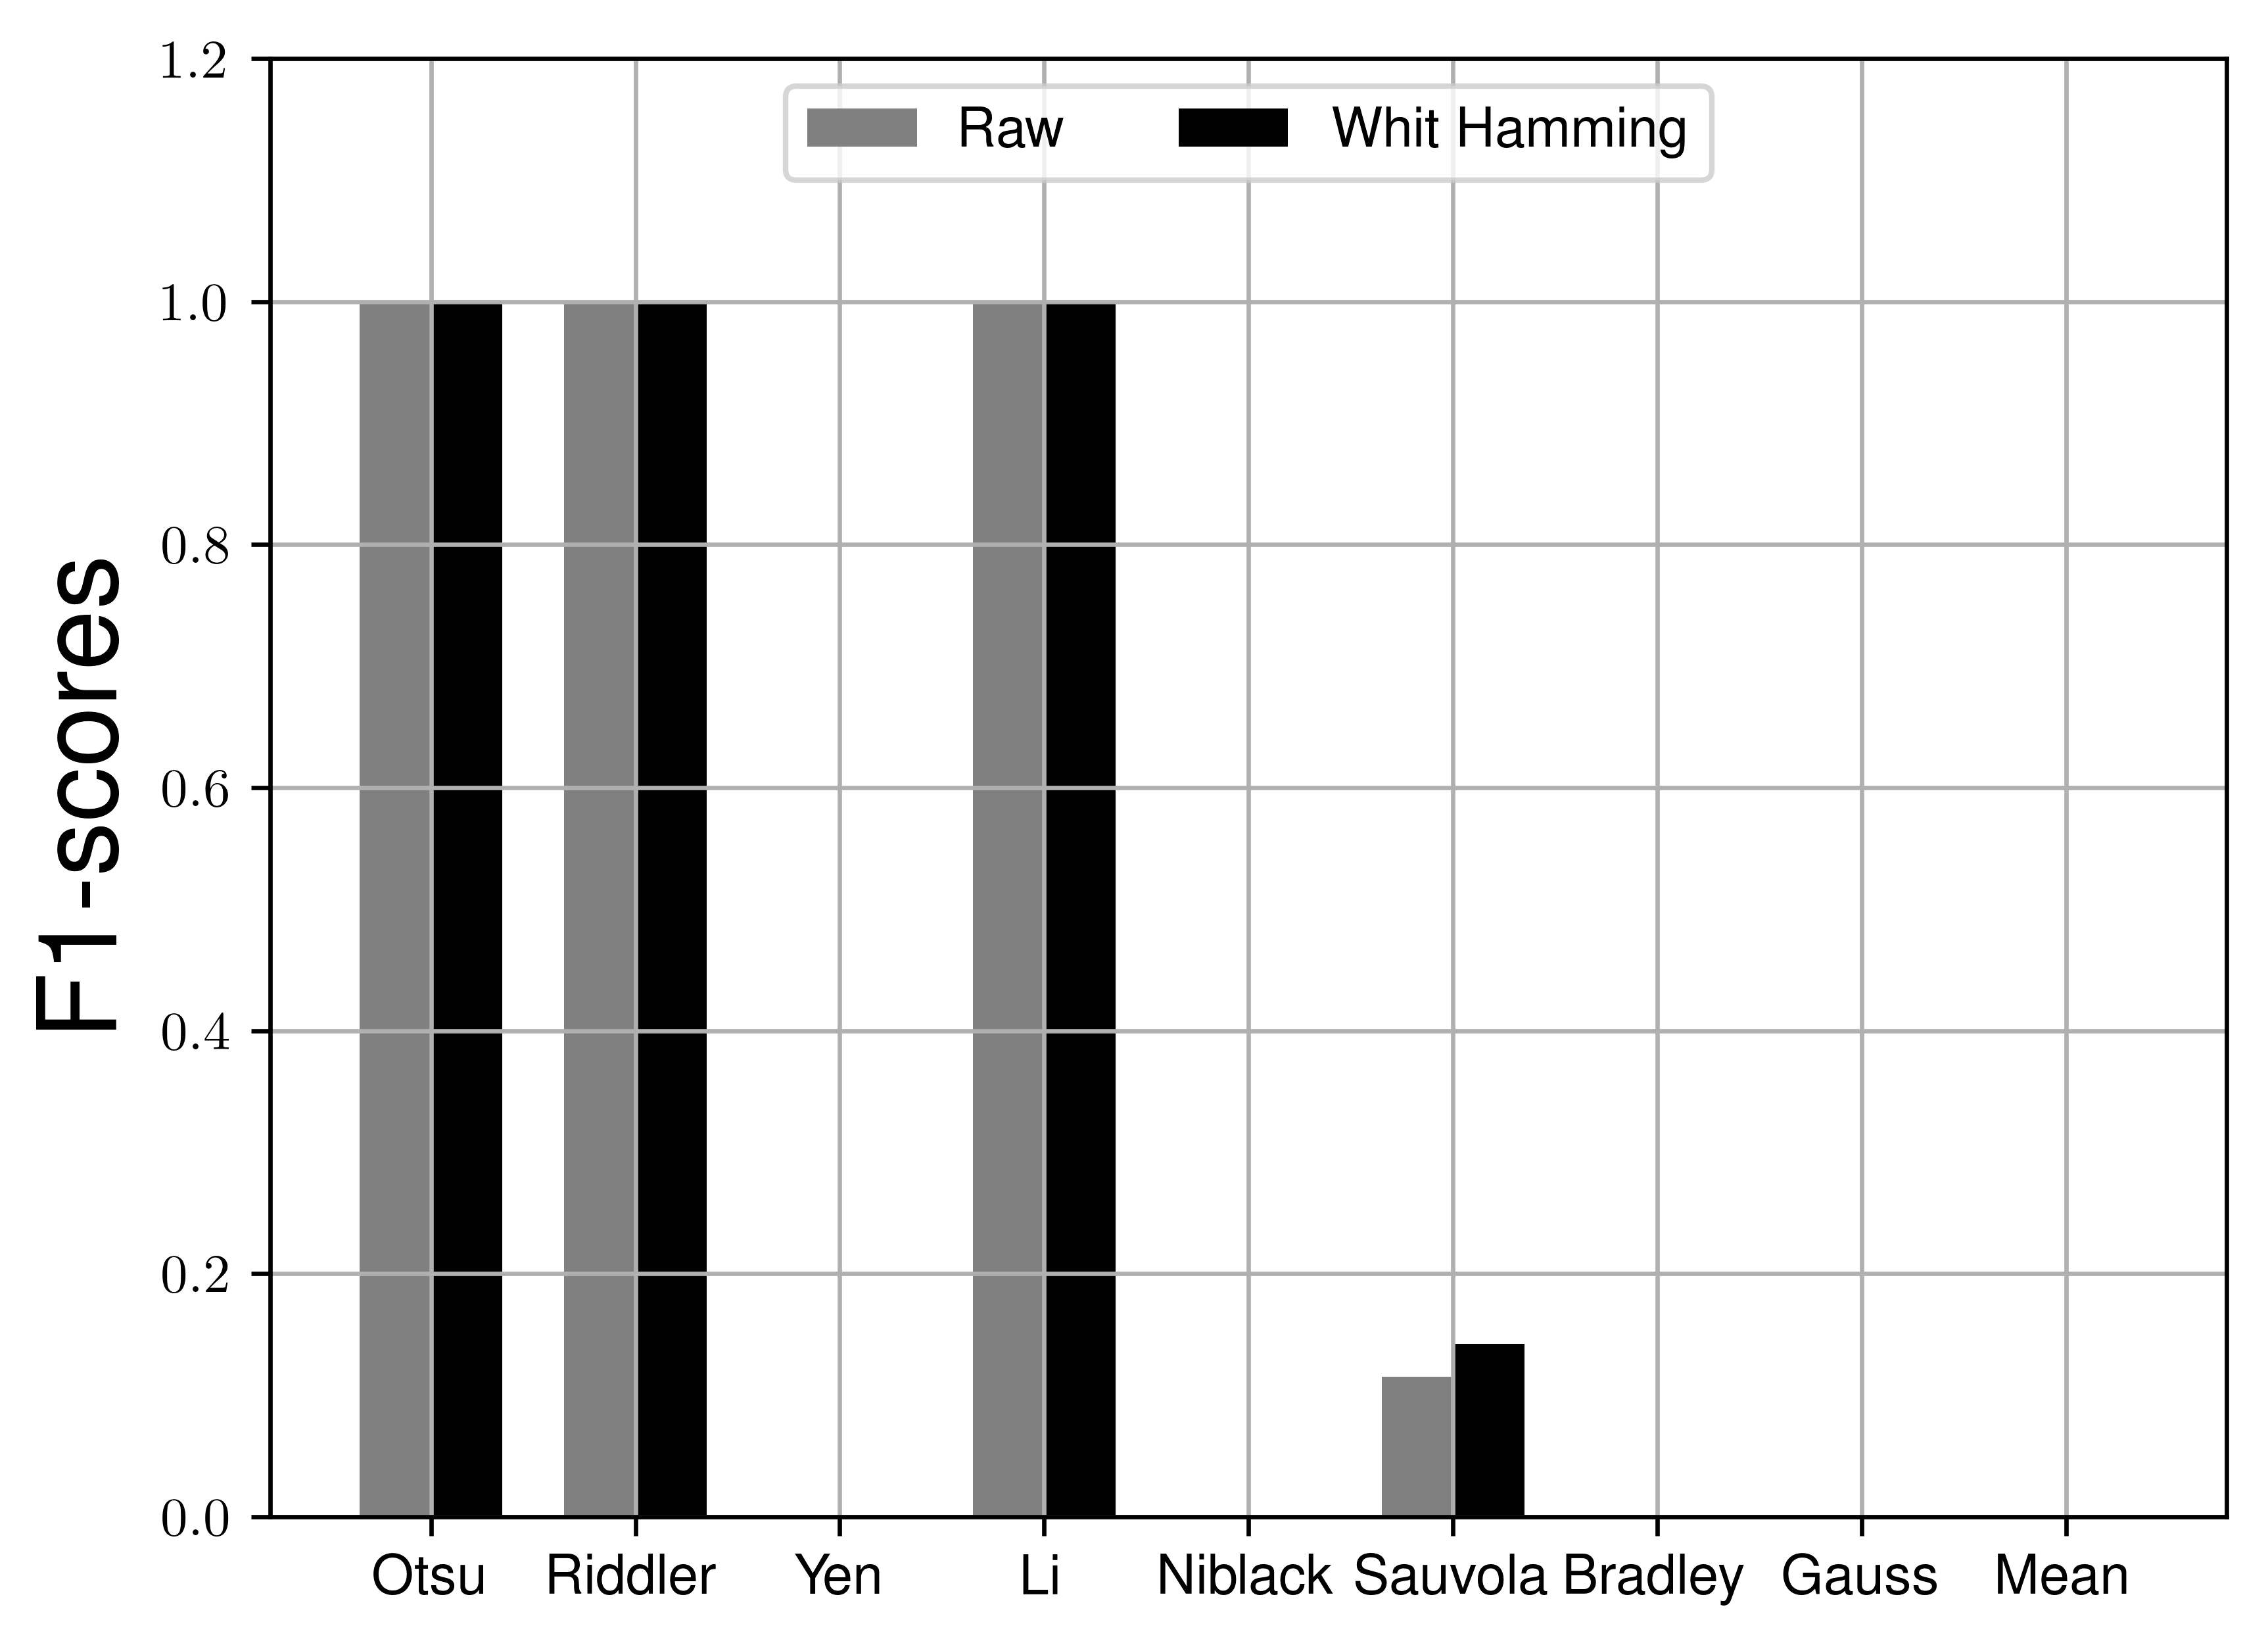
\includegraphics[width=\textwidth]{noise_comparison}
        \caption{}
        \label{fig:noise_graph}
    \end{subfigure}
        ~ %add desired spacing between images, e. g. ~, \quad, \qquad, \hfill etc. 
      %(or a blank line to force the subfigure onto a new line)
    \begin{subfigure}[b]{0.4\textwidth}
        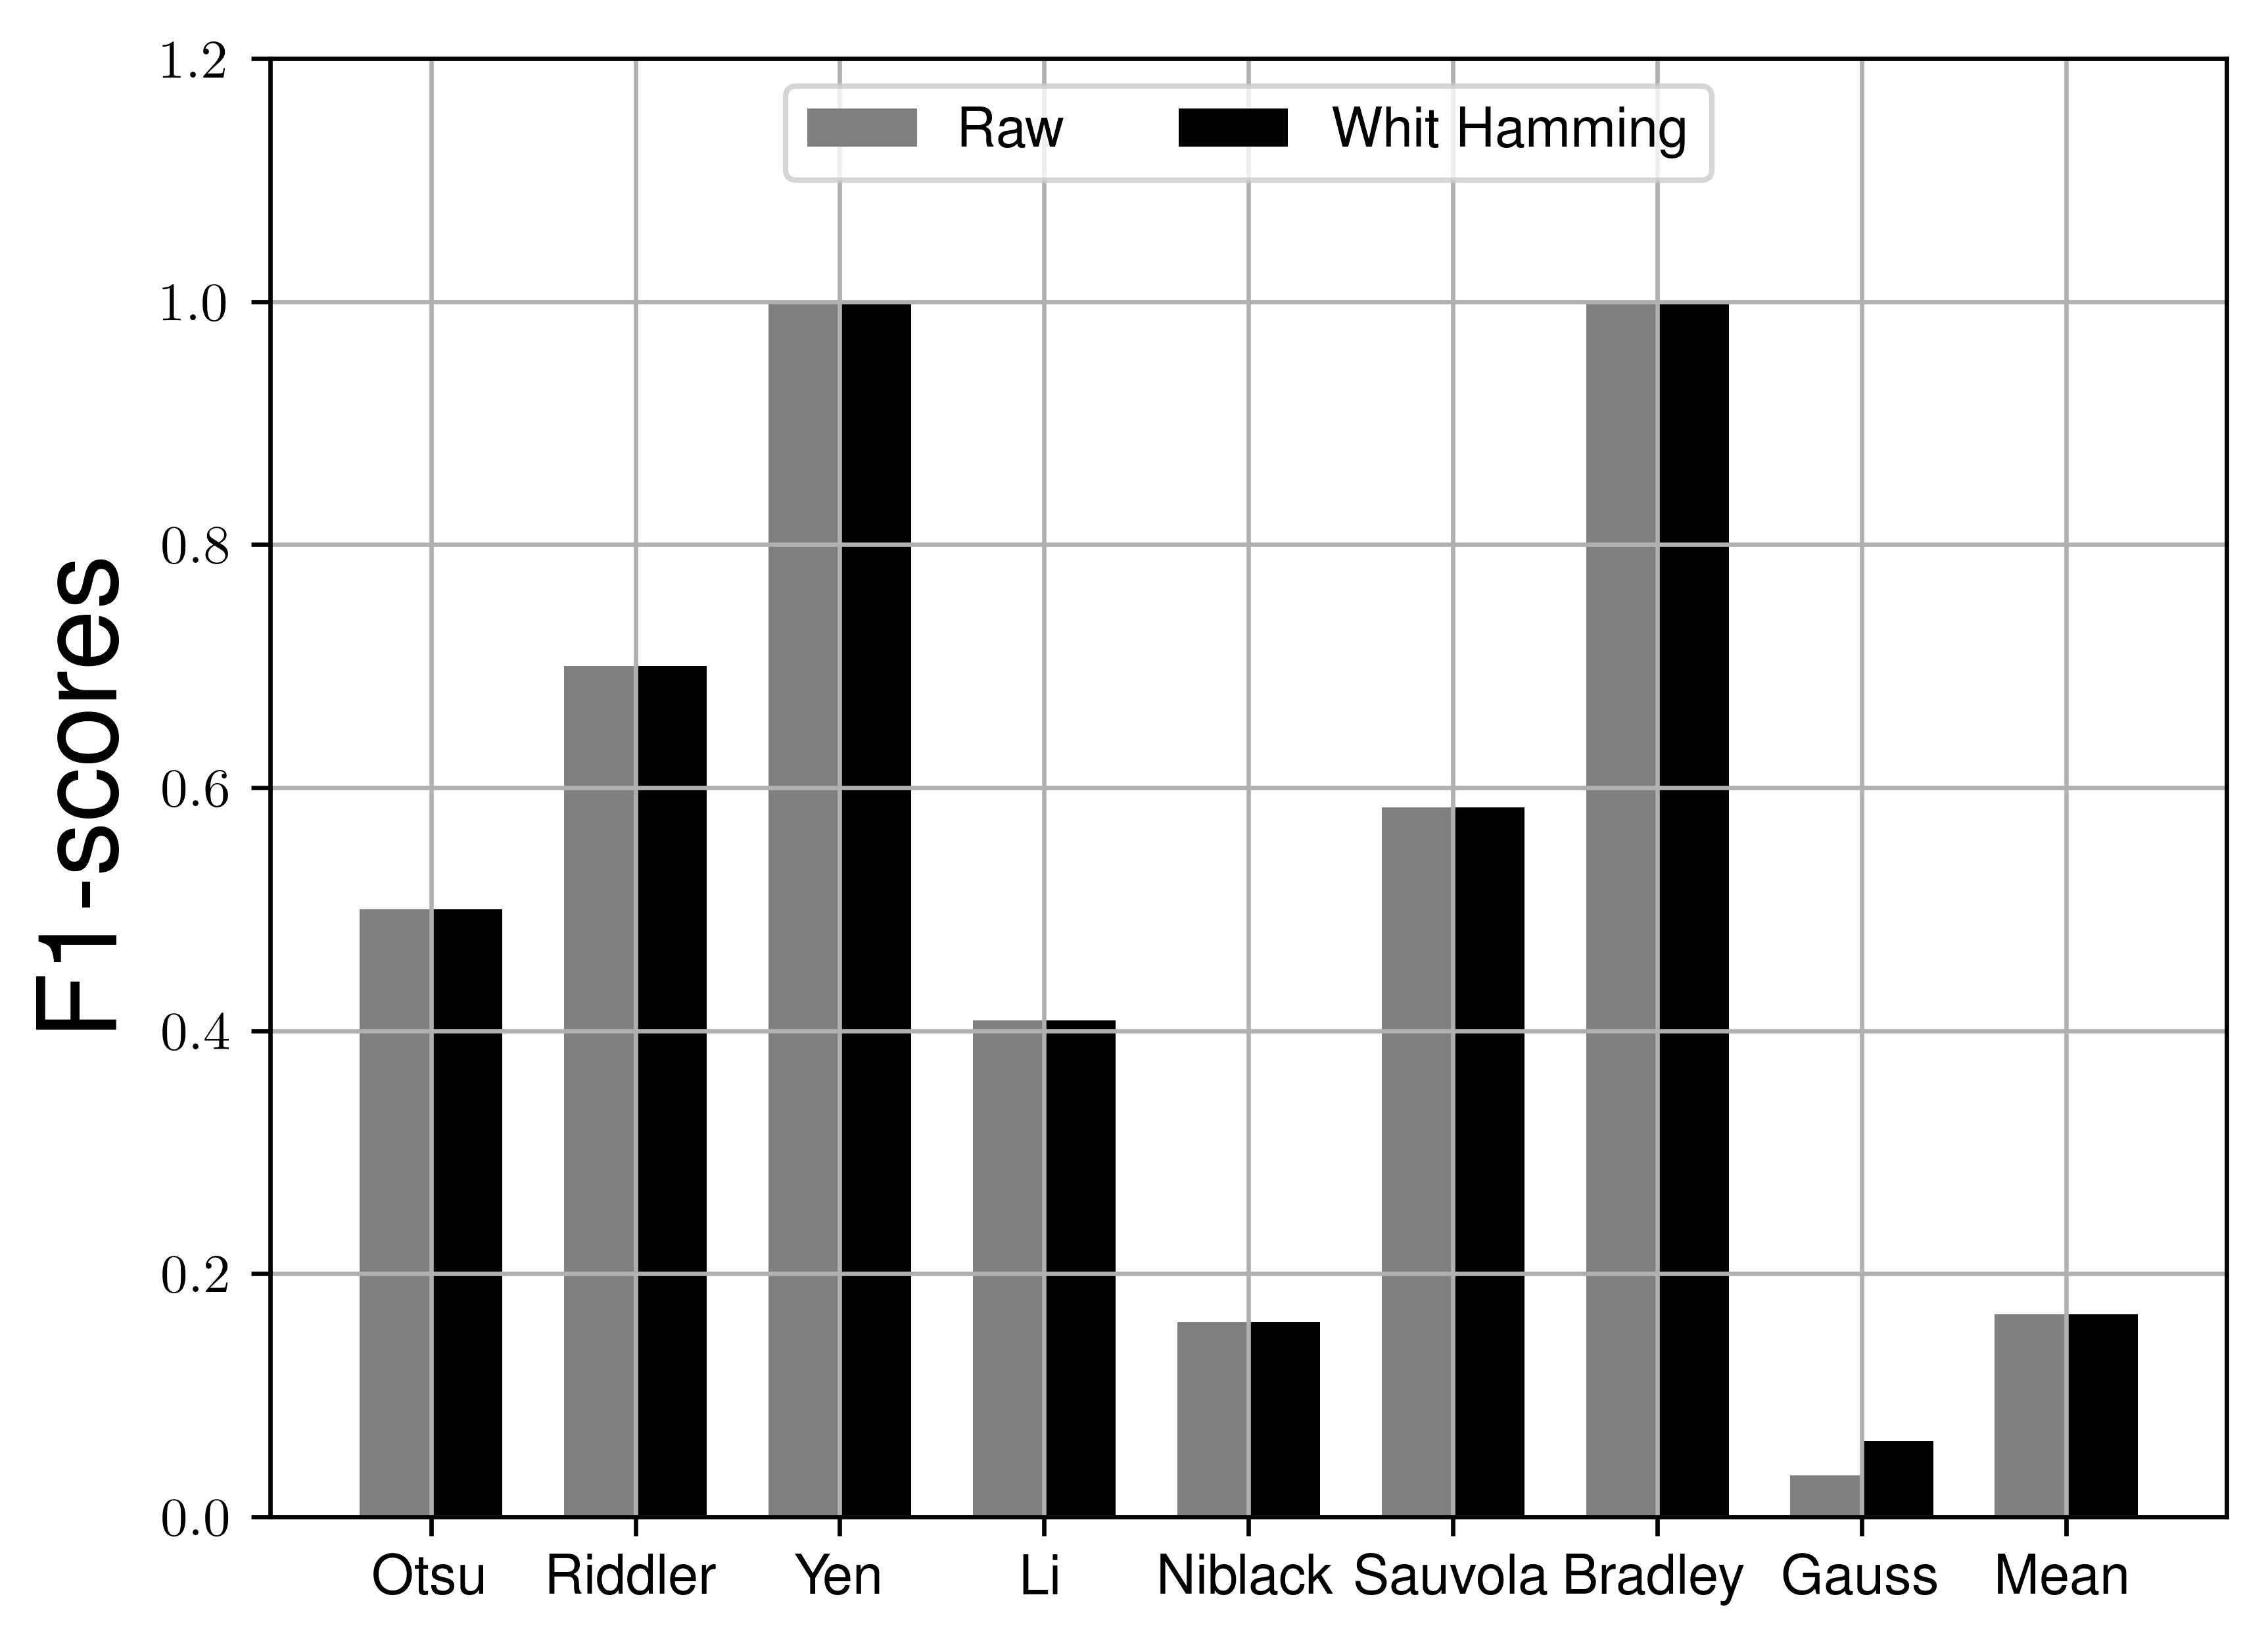
\includegraphics[width=\textwidth]{shade_comparison}
        \caption{}
        \label{fig:shadow_graph}
    \end{subfigure}\\
        ~ %add desired spacing between images, e. g. ~, \quad, \qquad, \hfill etc. 
      %(or a blank line to force the subfigure onto a new line)
    \begin{subfigure}[b]{0.4\textwidth}
        \includegraphics[width=\textwidth]{resolution_comparison}
        \caption{}
        \label{fig:esolution_graph}
    \end{subfigure}
        ~ %add desired spacing between images, e. g. ~, \quad, \qquad, \hfill etc. 
      %(or a blank line to force the subfigure onto a new line)
    \begin{subfigure}[b]{0.4\textwidth}
        \includegraphics[width=\textwidth]{ellipse_comparison}
        \caption{}
        \label{fig:deformation_graph}
    \end{subfigure}
    \caption{F1-score bar graphs: \textbf{(a)} Noise, \textbf{(b)} Shadow, \textbf{(c)} Change of size and \textbf{(d)} Perspectice deformation}\label{fig:degradations_graphs}
\end{figure}

The figure \ref{fig:thresholding_comp} and the F1-score graphs (Fig. \ref{fig:degradations_graphs}) shows that given the conditions where a landing target can be found, no threshold-based method was robust to the set of perturbations. It is necessary to adjust parameters according to the condition to have acceptable results. Besides, we aim to recognize the landing targets in natural images where none, one or more landing targets can be present and the degradations are not isolated. The figure \ref{fig:input_image} shows a landing target in an outdoor environment where the four degradations depicted in figure \ref{fig:tar_degradations} are present. We also show his histogram to highlight the saturation levels of the scene and the contours obtained with a representative method of each class of the taxonomy in \citep{Sezgin.Sankur:EI:2010}: clustering-based (Fig. \ref{fig:otsu_th}), entropy-based (Fig. \ref{fig:li_th}), spacial (Fig. \ref{fig:gauss_th}) and local (Fig. \ref{fig:sauvola_th}) threshold-based methods.

\begin{figure}[!ht]
    \centering
    \begin{subfigure}[b]{0.3\textwidth}
        \frame{\includegraphics[width=\textwidth]{in_img_tar4}}
        \caption{Input image}
        \label{fig:input_image}
    \end{subfigure}
    ~ %add desired spacing between images, e. g. ~, \quad, \qquad, \hfill etc. 
      %(or a blank line to force the subfigure onto a new line)
    \begin{subfigure}[b]{0.3\textwidth}
        \includegraphics[width=\textwidth]{histogram}
        \caption{Histogram of input image}
        \label{fig:histogram}
    \end{subfigure}\\
        ~ %add desired spacing between images, e. g. ~, \quad, \qquad, \hfill etc. 
      %(or a blank line to force the subfigure onto a new line)
    \begin{subfigure}[b]{0.16\textwidth}
        \frame{\includegraphics[width=\textwidth]{in_img_tar4_zoom}}
        \caption{Zoom}
        \label{fig:tar4_zoom}
    \end{subfigure}
        ~ %add desired spacing between images, e. g. ~, \quad, \qquad, \hfill etc. 
      %(or a blank line to force the subfigure onto a new line)
    \begin{subfigure}[b]{0.16\textwidth}
        \frame{\includegraphics[width=\textwidth]{Otsu_cont}}
        \caption{Otsu}
        \label{fig:otsu_th}
    \end{subfigure}
        ~ %add desired spacing between images, e. g. ~, \quad, \qquad, \hfill etc. 
      %(or a blank line to force the subfigure onto a new line)
    \begin{subfigure}[b]{0.16\textwidth}
        \frame{\includegraphics[width=\textwidth]{Li_cont}}
        \caption{Li}
        \label{fig:li_th}
    \end{subfigure}
        ~ %add desired spacing between images, e. g. ~, \quad, \qquad, \hfill etc. 
      %(or a blank line to force the subfigure onto a new line)
    \begin{subfigure}[b]{0.16\textwidth}
        \frame{\includegraphics[width=\textwidth]{Gauss_cont}}
        \caption{Gauss }
        \label{fig:gauss_th}
    \end{subfigure}
        ~ %add desired spacing between images, e. g. ~, \quad, \qquad, \hfill etc. 
      %(or a blank line to force the subfigure onto a new line)
    \begin{subfigure}[b]{0.16\textwidth}
        \frame{\includegraphics[width=\textwidth]{Sauvola_cont}}
        \caption{Sauvola}
        \label{fig:sauvola_th}
    \end{subfigure}
    \caption{Landing target under non-controlled illumination conditions and the controus obtained with some threshold-based methods}\label{fig:thresholding_comp}
\end{figure}


\section{Unsupervised Perception Model}\label{sec:unsupervised_perception_model}
%
\subsection{Non-accidentalness Estimation}\label{subsec:Helmholtz}

\subsubsection{Contour Detection}\label{subsubsec:muiltiscale}

After the development of a first algorithm by \citep{BaquedanoA.:ESIEE:2017}, we take some elements of this work to develop a more general approach that explores the principles of human perception. Precisely, we keep the concept of concentric circle patterns for the generation of landing target (see appendix \ref{ch:target_description} for the description of the landing targets generation) and the use of images contours as input data.

Instead of using a threshold-based method, we obtain the image without fixing any parameter. The use of the Marr-Hildreth \citep{Marr.Hildreth:PRS:1980} operator guarantees to find continuous and closed contours eliminating the possible noise in the image, while the contours of objects remain unchanged in the presence of shadows. This technique convolves the intensity image $f$ with the 2-D Laplacian of Gaussian operator $\nabla^{2} G(x, y,\sigma)$ and generates an image, 
\begin{eqnarray}\label{eq:LoG}
l_\sigma =  \nabla^{2} G(\sigma)\ast f
\end{eqnarray}
in which we localize the zero-crossings. 

The parameter $\sigma$ in eq. (\ref{eq:LoG}) permits to control the amount of image smoothing, but also acts as scale parameter, that when varies, it generates different scale-space images. Since no single filter can be optimal simultaneously at all scales \citep{Marr.Hildreth:PRS:1980}, we use a multi-scale analysis \citep{Witkin:ICASSP:1984} to detect the zero-crossings in $l_\sigma$ at different scale-spaces to minimize the risk that some contour of interest is not detected. The image $l_\sigma$ from eq. (\ref{eq:LoG}) contains a set of contours $\mathcal{L}_{\sigma}=\{L_{i}^{\sigma}, \enspace i=0, 1, \ldots, N\}$ for a given scale $\sigma$. Then, 
\begin{eqnarray}\label{eq:all_ctns_set}
\mathcal{L}=\bigcup\limits_{\sigma}  L_{\sigma}
\end{eqnarray}
represents all the contours of an image obtained at different scale-spaces. Figure \ref{fig:all_cnts} shows the set of contours $\mathcal{L}$ found for $\sigma=[1,2,3]$. Besides, it is also appreciated that at a fine scale (Fig. \ref{fig:cnts_scale1}) we can see more characteristics of the objects, i.e., there are more contours. Conversely, in coarse scales (Fig. \ref{fig:cnts_scale3}), due to the smoothing, there is a spatial distortion, and fewer contours appear. However, those contours that had already appeared at a coarse scale, will not disappear. Then, exist the probability that those contours that spatially coincide on two or more scales belong to a change of intensity generated by the border of an object. 

\begin{figure}[!ht]
    \centering
    \begin{subfigure}[b]{0.3\textwidth}
        \frame{\includegraphics[width=\textwidth]{cnts_sig1_tar4}}
        \caption{$\mathcal{L}_{\sigma}$ for $\sigma=1$}
        \label{fig:cnts_scale1}
    \end{subfigure}
    ~ %add desired spacing between images, e. g. ~, \quad, \qquad, \hfill etc. 
      %(or a blank line to force the subfigure onto a new line)
    \begin{subfigure}[b]{0.3\textwidth}
        \frame{\includegraphics[width=\textwidth]{cnts_sig3_tar4}}
        \caption{$\mathcal{L}_{\sigma}$ for $\sigma=2$}
        \label{fig:cnts_scale2}
    \end{subfigure}\\
        ~ %add desired spacing between images, e. g. ~, \quad, \qquad, \hfill etc. 
      %(or a blank line to force the subfigure onto a new line)
    \begin{subfigure}[b]{0.3\textwidth}
        \frame{\includegraphics[width=\textwidth]{cnts_sig3_tar4}}
        \caption{$\mathcal{L}_{\sigma}$ for $\sigma=3$}
        \label{fig:cnts_scale3}
    \end{subfigure}
        ~ %add desired spacing between images, e. g. ~, \quad, \qquad, \hfill etc. 
      %(or a blank line to force the subfigure onto a new line)
    \begin{subfigure}[b]{0.3\textwidth}
        \frame{\includegraphics[width=\textwidth]{all_cnts_tar4}}
        \caption{Set $\mathcal{L}$ for $\sigma=[1, 2 ,3]$}
        \label{fig:all_cnts}
    \end{subfigure}
    \caption{The image contours found at three different scales joined in the set $\mathcal{L}$}\label{fig:multiscale_cnts}
\end{figure}

\subsubsection{Multi-feature Space}\label{subsec:multispace}
The Helmholtz principle states that meaningful characteristics appear as large deviations from randomness and that is how the human perception automatically works to identify an object \citep{Attneave:PR:1954}. The a contrario model proposed in \citep{Desolneux.Moisan.ea:Gestalt:2008}, formulates this principle statistically by setting the number of false alarms (NFA) below some acceptable level; however, this method cannot be easily extended to more complex shapes. Instead of setting the NFA, we use the RX detector \citep{Reed.Yu:TASSP:1990} to detect outliers. Initially called the constant false alarms rate detection algorithm (CFAR) it can detect the presence of a know signal pattern in several signal-plus-noise channels. For that, it uses a $N\times Q$ multi-variable space $Z=[Z_{1}, \ldots, Z_{Q}]$ with $Q$  observation vectors of dimension $N$. In our approach, the primitive is a closed contour. We build the multi-variable space with observations based on internal (geometrical features, e.g., circularity, roundness, area, perimeter) and external (e.g., mean gradient intensity,  intensity inner area) properties of the contours.

Let $L_{i} \in \mathcal{L}$ be a contour, $A_{i}$ its area and $P_{i}$ its perimeter; we compute the circularity eq.(\ref{eq:circuarity}) and the mean gradient intensity eq. (\ref{eq:mean_gradient}) to build the multi-variable space $Z=[Z_{1}, Z_{2}]$. 

\begin{eqnarray}
Z_{1}&=&\left[\frac{4\pi A_{i}}{P_{i}^2}, \enspace i=0, \ldots, N\right]^T,  \enspace N = card(\mathcal{L}) \label{eq:circuarity}  \\ 
Z_{2}&=&\left[\frac{1}{P_{i}}\sum\limits_{x \in L_{i}} \mid\nabla f(x) \mid, \enspace L_{i} \in \mathcal{L}\right]^T  \label{eq:mean_gradient}
\end{eqnarray}

\subsubsection{RX Detector}\label{subsec:rx_detector}
The RX anomaly detector \citep{Reed.Yu:TASSP:1990} is commonly used to detect outliers on such data. The space $Z$ models the set of contours $\mathcal{L}$ with $Q=2$ feature vectors describing the circularity eq. (\ref{eq:circuarity}) and the mean gradient intensity eq.(\ref{eq:mean_gradient}). The RX detector gives an anomaly score to each contour taking into account the mean of the distribution and covariance between the $Q$-features through the Mahalanobis distance,
\begin{eqnarray}\label{eq:RX_detector}
y_{i}= (z_{i}-\mu_{Z})^{T}\Sigma^{-1}_{Z}(z_{i}-\mu_{Z})
\end{eqnarray}
where $\mu_{Z}=[\mathrm{E}[z_{1}], \ldots, \mathrm{E}[z_{N}]]^T$ is the  observations mean vector and $\Sigma^{-1}_{Z}$ the $N\times Q$ covariance matrix of the data. If the data have normal random distribution, then the score vector $Y=[y_{i}, \ldots, y_{N}]$ follows a chi-square distribution $\chi^{2}_{Q}(\varphi)$ with $Q$ degrees of freedom, where $\varphi$ is a confidence level \citep{Lu.Chen.ea:IJAIT:2004}. The value of $\chi^{2}_{Q}(\varphi)$ with a confidence value $\varphi=99.9\%$ operates as a threshold to identify all contours that behave as outliers in the multi-variable distribution. In our case, the contours belonging to a landing target appear as outliers in the vast majority of random contours belonging to the background.

With the previous strategy we preserve the anomalous contours having a value of mean gradient and circularity deviating from the principal mode of the distribution in the set $\widetilde{\mathcal{L}}=\{L_{i}\mid y_{i}>\chi^{2}_{Q}(\varphi)\}$. $\chi^{2}_{Q}(\varphi)$ is the value of the cumulative distribution at the confidence level $\varphi$ and $\widetilde{\mathcal{L}} \subset \mathcal{L}$. It is essential to mention the importance of multi-scale contour detection of section \ref{subsec:multispace}; because it increases the number of samples in Z, allowing to build a richer multi-variable space.

In the set $\widetilde{\mathcal{L}}$ some contours make not part of a landing target. For example, in the figure \ref{fig:rx_cnts}, we can see that the paper sheet contours remain because they have a high value of circularity. The same occurs with the contours of those objects with an important value of mean gradient, as the number 4 at the top-left of the sheet or the rock textures of the background.
\begin{figure}[h]
    \centering
    \frame{\includegraphics[width=0.35\linewidth]{rx_cnts_tar4}}
    \caption{The contours from Fig. \ref{fig:all_cnts} that behave as outliers in the multi-feature space $Z$ with a confidence value of $\varphi=99.9\%$}
    \label{fig:rx_cnts}
\end{figure}

\subsection{Gestalt Laws of Grouping}\label{subsec:Gestalt}
We use the Gestalt theory \citep{Wertheimer:Psycologische:1923} to group the meaningful contours $L_{i}\in \widetilde{\mathcal{L}}$ and detect landing targets.

\subsubsection{Goodness of Shape}\label{subsec:similarity}
Since the landing targets have only circular contours, we evaluate the resemblance with an ellipse (to deal with the perspective deformation) of all contours. Considering an ellipse $e_{i}$ that fits one gray contour $L_{i}$ in figure \ref{fig:affinity}, we recover the centroid $C_{i}$, the rotational angle $\rho$, the semi-major axis $\alpha_i$, the semi-minor axis $\beta_{i}$ and the coordinates $F_{i}$ and $F_{i}'$ of the ellipse's foci. Then, the sum of the distances from any point of ellipse $x_{j}\in e_{i}$ to the foci is $\overline{x_{j}F_{i}}+\overline{x_{j}F_{i}'}=2\alpha_{i}$. If the contour $L_{i}$ is an ellipse, the value $d_{i}=\abs{(\overline{x_{j}F_{i}}+\overline{x_{j}F_{i}'})-2\alpha_{i} }$ must be zero or negligible $\forall x_{j}\in L_{i}$. 

\begin{figure}[h]
    \centering
    \begin{subfigure}[b]{0.4\textwidth}
        \includegraphics[width=\textwidth]{affinity_ellipse}
        \caption{Affinity of a fit $\omega_{i}$}
        \label{fig:affinity}
    \end{subfigure}
    ~ %add desired spacing between images, e. g. ~, \quad, \qquad, \hfill etc. 
      %(or a blank line to force the subfigure onto a new line)
    \begin{subfigure}[b]{0.45\textwidth}
        \includegraphics[width=\textwidth]{DoA_ellipse}
        \caption{Difference of area $\Delta_{A_{i}}$}
        \label{fig:DoA}
    \end{subfigure}\\
    \caption{Visual description of affinity of ellipse and difference of area}\label{fig:ressemblance_ellipse}
\end{figure}

Based on the form of the landing target we estimate the the similarity using two measures, 
\begin{eqnarray}
\omega_{i}&=&\exp^{-\frac{d_{i}^{2}}{2\sigma^{2}}}\enspace \mbox{the affinity of the fit and,}\label{eq:GoE}\\
\Delta_{A_{i}}&=& 1-\frac{\abs{ A_{e_{i}}-A_{i}}}{\max(A_{e_{i}},A_{i})} \enspace \mbox{the difference of area.}\label{eq:DoA}
\end{eqnarray}

The affinity $\omega_{i}\rightarrow 1$ for contours closed to an ellipsoidal shape. However, if the contour $L_{i}$ is a croissant shape (as in fig. \ref{fig:DoA}) then, the eq. (\ref{eq:GoE}) also has a high value (near to 1) but the contour is from being an ellipse. The variable in eq. (\ref{eq:DoA}) complements the affinity $\omega_{i}$ taking into account the area of the ellipse $A_{e_{i}}$ and the area of the contour $A_{i}$. To calculate the similarity to an ellipse, we use the harmonic mean of both. 
\begin{eqnarray}
\kappa_{i}&=&\mathcal{H}(\omega_{i}, \Delta_{A_{i}}), \enspace \kappa_{i}\in (0,1)\label{eq:similarity}
\end{eqnarray}
where $\kappa_{i}\rightarrow 1$ for contours ressembling to an ellipse and $\kappa_{i}\rightarrow 0$ otherwise. $\mathcal{H}$ denotes the harmonic mean $\mathcal{H}= N \left(\sum\limits_{i=1}^{N} \xi_{i}^{-1} \right)^{-1}$.

\subsubsection{Proximity Measure}\label{subsec:proximity}
The Gestalt law of proximity states that we group those meaningful elements if they are spatially close to each other. In the case of contours, we take the coordinates of their centers $C_{i}$ to measure their spatial proximity.

\subsubsection{Affinity Clustering}\label{subsec:clustering}
The normalized coordinates of the centroid $C_i$ and the ellipse similarity $\kappa_i$ map the contour $L_i\in \widetilde{\mathcal{L}}$ into the 3-D space $(0,1) \in \mathbb{R}^3$. We use the affinity propagation clustering method \citep{Frey.Dueck:SCIENCE:2017} to group the contours using the matrix $X=[C_{i}, \kappa_{i}]$. This technique yields a set of clusters $\mathcal{C}_{K}\in \mathcal{C}(X)$. Because the landing target has ten different contours (see apendix \ref{ch:target_description}), the clusters with $card(\mathcal{C}_{K})\geq 10$ and an important similarity value $\mathcal{H}(\kappa_{i})\geq 0.8$, represent the candidate contours of a landing target.

\begin{figure}[h]
    \centering
    \begin{subfigure}[b]{0.3\textwidth}
        \includegraphics[width=\textwidth]{3dplot_tar4}
        \caption{Clusters obtained by affinity propagation}
        \label{fig:3dplot}
    \end{subfigure}
    ~ %add desired spacing between images, e. g. ~, \quad, \qquad, \hfill etc. 
      %(or a blank line to force the subfigure onto a new line)
    \begin{subfigure}[b]{0.3\textwidth}
        \includegraphics[width=\textwidth]{2dplot_xy_tar4}
        \caption{ Clusters projected on the image domain}
        \label{fig:2dplot}
    \end{subfigure}
    ~ %add desired spacing between images, e. g. ~, \quad, \qquad, \hfill etc. 
      %(or a blank line to force the subfigure onto a new line)
    \begin{subfigure}[b]{0.3\textwidth}
        \includegraphics[width=\textwidth]{2dplot_candidate_tar4}
        \caption{Target candidate cluster}
        \label{fig:candidate}
    \end{subfigure}
   \caption{Clusters of contour from Fig. \ref{fig:rx_cnts}}\label{fig:grouping_process}
\end{figure}

The affinity propagation technique groups in $K=12$ clusters the image contours from figure \ref{fig:rx_cnts}. In a 3D plot (fig. \ref{fig:3dplot}), we see the influence of $\kappa_{i}$ at clustering process. Projecting the clusters in a 2-D plane (fig. \ref{fig:2dplot}), we notice that even if the contours are nearby, it can form a new cluster if there is a distant $\kappa$. A clear example is the clusters 0 and 4 (blue and purple, respectively) that correspond to the contour centers of the landing target and the center of the sheet of paper, they are close to each other but the similarity not. Applying the threshold values $card(\mathcal{C}_{K})\geq 10$ and $\mathcal{H}(\kappa_{i})\geq 0.8$ we obtain the candidate clusters to form a landing target (see fig.~\ref{fig:candidate}). 

Heretofore, we have built a model based on perceptual characteristics for the landing target detection. However, there could be false detections if there are round objects with concentric borders in the image. We code an ID number in the target design to differentiate a landing target from an object with concentric circular edges. The coding of information allows discriminating between several landing targets and circular objects. The following section describes the landing target design as well as the coding and decoding technique. 

\section{Model Vadilation and Test}\label{sec:validation_and_test}
The presented strategy was validated on landing target images under simulated and real situations. We tested the algorithm in a synthetic image database which simulates four image degradations: noise, shadows, target deformation and change of size. For the real situations, we carried out several tests in indoor and outdoor scenarios. Figure \ref{fig:validation} shows three interesting experiments and the output image of each stage of section \ref{sec:perception_model}. 

\begin{figure}[h!]
\centering
\begin{subfigure}[t]{\dimexpr0.30\textwidth+20pt\relax}
    \makebox[20pt]{\raisebox{40pt}{\rotatebox[origin=c]{90}{Set $\mathcal{L}$}}}%
    \frame{\includegraphics[width=\dimexpr\linewidth-20pt\relax]
    {all_cnts_synthetic_tar14}}
    \makebox[20pt]{\raisebox{40pt}{\rotatebox[origin=c]{90}{Set $\widetilde{\mathcal{L}}$}}}%
    \frame{\includegraphics[width=\dimexpr\linewidth-20pt\relax]
    {rx_cnts_synthetic_tar14}}
    \makebox[20pt]{\raisebox{40pt}{\rotatebox[origin=c]{90}{Clusters $\mathcal{C}_{K}$}}}%
    \frame{\includegraphics[width=\dimexpr\linewidth-20pt\relax]
    {cnts_cluster_synthetic_tar14}}
    \makebox[20pt]{\raisebox{40pt}{\rotatebox[origin=c]{90}{Result}}}%
    \frame{\includegraphics[width=\dimexpr\linewidth-20pt\relax]
    {synthetic_tar14}}
    \caption{} \label{fig:synthetic_result}
\end{subfigure}\hfill
\begin{subfigure}[t]{0.30\textwidth}
    \frame{\includegraphics[width=\textwidth]
    {all_cnts_16tar}}
    \frame{\includegraphics[width=\textwidth]
    {rx_cnts_16tar}}
    \frame{\includegraphics[width=\textwidth]
    {cnts_cluster_16tar}}
    \frame{\includegraphics[width=\textwidth]
    {16tar}}
    \caption{} \label{fig:indoor_result}
\end{subfigure}\hfill
\begin{subfigure}[t]{0.30\textwidth}
    \frame{\includegraphics[width=\textwidth]
    {all_cnts_5tar2}}
    \frame{\includegraphics[width=\textwidth]
    {rx_cnts_5tar2}}
    \frame{\includegraphics[width=\textwidth]
    {cnts_cluster_5tar2}}
    \frame{\includegraphics[width=\textwidth]
    {5tar2}}
    \caption{}  \label{fig:outdoor_result}
\end{subfigure}
\caption{Algorithm validation: (a) Target under simulated degradations, (b) The 16 targets in an indoor environment, (c) Five targets in an outdoor scenario under non-controlled image degradations}\label{fig:validation}
\end{figure}

The first experiment (Fig. \ref{fig:synthetic_result}) shows the four synthetic degradations together on landing target ID 14. In this context, the synthetic image represents the values of degradation maximum that the algorithm supports. The second experiment (Fig. \ref{fig:indoor_result}) was done in an indoor space to show the sixteen possible landing targets. In the scene, there are no other objects. Finally, the last experiment (Fig. \ref{fig:outdoor_result}) shows five landing targets in a more complex outdoor environment. Notice the presence of other objects, different background textures,  irregular shadows and perspective deformation and change of scale of the landing targets. 

In the three experiments, i) the non-accidentalness estimation stage eliminates the contours generated by noise with low circularity and mean gradient values; ii) the grouping stage filters random contours generated by intensity changes like shadows to keep contours with an important value of similarity and proximity. The compilation of the experiments carried out under real conditions can be seen in \url{https://youtu.be/igsQc7VEF2c}.

\section{Conclusion}\label{sec:conclusions_landing_target}
In this chapter we have described two procedure for the landing target detection and recognition. The first one, in section \ref{sec:hierarchical_target_detection}, using a straightforward hierarchical method and the second one, in section \ref{sec:unsupervised_perception_model}, based on a perception model. The second algorithm is based on the Helmholtz non-accidentalness principle and the Gestalt theory. The non-accidentalness estimation is performed in a multi-feature object space built from the image contours at different scales. This approach allows us to obtain scene information avoiding the loss of information because of the objects' change of size or the presence of shadows and noise and the change of perspective. We have used the similarity and proximity Gestalt laws to group the contours and build a perceptual object and the Hamming error codes to perform the landing target recognition. The experiments show that the proposed methodology for the detection of landing targets is robust to uncontrolled light conditions and other images degradations existing in complex environments.

With this framework, we tackle one of the specific tasks proposed in section \ref{sec:objectives_of_the_thesis}, the target detection and identification. So far, we have only considered the contours and some internal/external observations to build a multi-variable space $Z$ to detect a geometric circular shape with concentric borders. 

%The importance of the study the image primitives in different levels of abstraction lies in the type of information we can retrieve and analyze. Table \ref{tab:primitives_features} shows hierarchically some image primitives and the information that we can have from them. Notice that as the primitive becomes complex, it posses more information. These fundamental features, also add other derivated features such as statistical moments, histogram, variance, frequency. Other features are more complex such as alignments, which derived from the position as a distance to a fitted line. 
%
%\begin{table}[!ht]
%\centering
%\begin{tabular}{|c|c|c|}
%\hline
%\textbf{Primitive} & \textbf{Endogenous Features}                                                                                                                            & \textbf{Exogenous Features}                                                                                          \\ \hline
%Point              & position                                                                                                                                                & \begin{tabular}[c]{@{}c@{}}intensity\\ gradient\end{tabular}                                                    \\ \hline
%Segment            & \begin{tabular}[c]{@{}c@{}}position\\ orientation\\ length\\ curvature\end{tabular}                                                                     & \begin{tabular}[c]{@{}c@{}}intensity\\ gradient\end{tabular}                                                    \\ \hline
%Contour/Region     & \begin{tabular}[c]{@{}c@{}}position\\ orientation\\ length\\ curvature\\ compactness\\ moments\\ surface area\\ perimeter\\ Feret diameter\end{tabular} & \begin{tabular}[c]{@{}c@{}}intensity\\ gradient\\ entropy\\ color\\ texture \end{tabular} \\ \hline
%\end{tabular}\caption{Principal image primitives and its internal and external features}\label{tab:primitives_features}
%\end{table}

In the next part of this thesis we will explore the global color and texture feautures of an image. The main idea is to retrieve the largest possible number of image primitives and features to build a multivariable space $Z$ (similar to section \ref{subsec:multispace}) that represent the objects in an image. We have already obtained some contour features that were used for the target detection. The proposition now is to use the distribution of color and texture to feed the multivariable space. 


\textbf{AI offers solutions but no answers, and we need both!!}